%----------------------------------------------------------------------------------------
%
% LaTeX-template for degree projects at LNU, Department of Computer Science
% Last updated by Johan Hagelbäck, Mar 2017
% Linnaeus University
%
% License: Creative Commons BY
%
%----------------------------------------------------------------------------------------

%----------------------------------------------------------------------------------------
%	Settings and configuration
%----------------------------------------------------------------------------------------

\documentclass[a4paper,12pt]{article}

\usepackage[T1]{fontenc}
\usepackage{times}
\usepackage[english]{babel}
\usepackage[utf8]{inputenc}
\usepackage{dtklogos}
\usepackage{wallpaper}
\usepackage[absolute]{textpos}
\usepackage[top=2cm, bottom=2.5cm, left=3cm, right=3cm]{geometry}
\usepackage{appendix}
\usepackage[nottoc]{tocbibind}
\usepackage[colorlinks=true,
            linkcolor=black,
            urlcolor=blue,
            citecolor=black]{hyperref}

\setcounter{secnumdepth}{3}
\setcounter{tocdepth}{3}

\usepackage{sectsty}
\sectionfont{\fontsize{14}{15}\selectfont}
\subsectionfont{\fontsize{12}{15}\selectfont}
\subsubsectionfont{\fontsize{12}{15}\selectfont}

\usepackage{csquotes} % Used to handle citations

\renewcommand{\thetable}{\arabic{section}.\arabic{table}}  
\renewcommand{\thefigure}{\arabic{section}.\arabic{figure}} 

%----------------------------------------------------------------------------------------
%	
%----------------------------------------------------------------------------------------
\newsavebox{\mybox}
\newlength{\mydepth}
\newlength{\myheight}

\newenvironment{sidebar}%
{\begin{lrbox}{\mybox}\begin{minipage}{\textwidth}}%
{\end{minipage}\end{lrbox}%
 \settodepth{\mydepth}{\usebox{\mybox}}%
 \settoheight{\myheight}{\usebox{\mybox}}%
 \addtolength{\myheight}{\mydepth}%
 \noindent\makebox[0pt]{\hspace{-20pt}\rule[-\mydepth]{1pt}{\myheight}}%
 \usebox{\mybox}}

%----------------------------------------------------------------------------------------
%	Title section
%----------------------------------------------------------------------------------------
\newcommand\BackgroundPic{
    \put(-2,-3){
    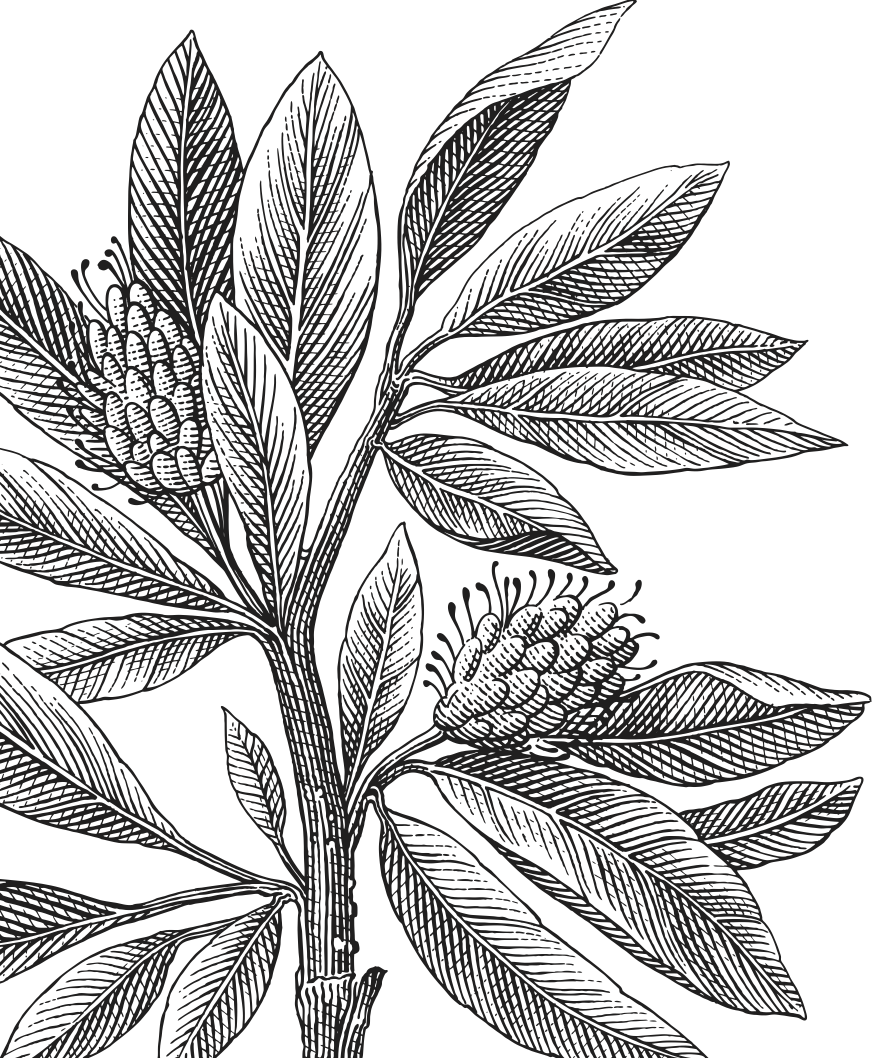
\includegraphics[keepaspectratio,scale=0.3]{img/lnu_etch.png} % Background picture
    }
}
\newcommand\BackgroundPicLogo{
    \put(30,740){
    
\includegraphics[keepaspectratio,scale=0.10]{img/logo.png} % Logo in upper left corner
    }
}

\title{	
\vspace{-8cm}
\begin{sidebar}
    \vspace{10cm}
    \normalfont \normalsize
    \Huge Bachelor Degree Project \\
    \vspace{-1.3cm}
\end{sidebar}
\vspace{3cm}
\begin{flushleft}
    \huge Relation between Linguistic quality and Design quality in RESTful APIs\\ 
\end{flushleft}
\null
\vfill
\begin{textblock}{6}(10,13)
\begin{flushright}
\begin{minipage}{\textwidth}
\begin{flushleft} \large
\emph{Authors:} Jesper Hägglund, Edvin Larsson\\ % Author
\emph{Supervisor:} Francis Palma \\ % Supervisor
%\emph{Examiner:} Dr.~Mark \textsc{Brown}\\ % Examiner (course manager)
\emph{Semester:} VT 2020\\ % 
\emph{Subject:} Computer Science\\ % Subject area
\end{flushleft}
\end{minipage}
\end{flushright}
\end{textblock}
}

\date{} 

\begin{document}
\pagenumbering{gobble}
\newgeometry{left=5cm}
\AddToShipoutPicture*{\BackgroundPic}
\AddToShipoutPicture*{\BackgroundPicLogo}
\maketitle
\restoregeometry
\clearpage
%----------------------------------------------------------------------------------------
%	Abstract
%----------------------------------------------------------------------------------------
\selectlanguage{english}
\begin{abstract}
REST API is one of the most common protocols for client/server communication in modern web. Earlier research has shown that quality of a REST API can be measured by linguistic and design rules. This research focus on the relationship between linguistic and design quality. Our goal is to raise the awareness among REST API developers to focus more on quality to make their APIs easier to use by following common standards. We have run  tests for detecting antipatterns that break these rules in 10 widely used apis over a total of 326 endpoints. Our conclusion is that there is an overall relationship between design and linguistic quality in REST APIs. However, more research is needed to fully validate the result and its accuracy.
\end{abstract}

\newpage
\pagenumbering{gobble}
\tableofcontents % Table of contents
\newpage
\pagenumbering{arabic}

%----------------------------------------------------------------------------------------
%
%	Here follows the actual text contents of the report.
%
%----------------------------------------------------------------------------------------

\section{Introduction}

\subsection{Background}
Representational State Transfer (REST) is a commonly used architectural pattern for designing Application Programming Interfaces (APIs). 

The popularity of REST has been increasing during the last two decades since its introduction in the year 2000 by Roy Fielding \cite{restdissertation}. Today the biggest tech companies like Twitter, Google, Dropbox - to name a few - utilizes REST APIs in their tech stack. 

When the big tech companies make their REST APIs public for other developers to use and integrate in their own applications it is important that their REST APIs adhere to common practices for ease of use and understandability. However, research by Palma et al. \cite{linguistic}\cite{design} has shown that APIs often deviate from the common practices. 

This study will investigate if there is a correlation between REST design quality and linguistic quality in RESTful APIs.

\subsection{Defining REST}

A REST API is an API that complies to REST architecture constraints. There are six REST architecture constraints as described by Roy Fielding \cite{restdissertation}, which will be explained from a HTTP protocol perspective:

\begin{enumerate}
\item Client-server. Separates the user interface from the data storage. This separation makes it possible for independent development of these components. 
\item Stateless. The client should do the session handling while the server remains stateless and does not store data about previous requests. This makes it possible to scale the server and recover from failures without the loss of data.
\item Cacheable. Each response to a GET request should be cacheable by the client. This is for reducing requests to server for more efficient delivery of resources and scaling. 
\item Uniform interface. REST defines four constraints to achieve a uniform interface: 
\begin{enumerate}
\item Identification of resources. A resource is anything that can be retrieved such as a document, image etc. Resource identification is usually done by URIs (uniform resource identifier).
\item Manipulation of resources through representation. This is a key-value pair that represents the resource. In HTTP this corresponds to request and response headers. Examples of headers are content-type, which defines type of resource (png, json), last-modified (timestamp of the last time a resource was modified).
\item Self-descriptive messages. Each message between the client and server should include all necessary information to take an  action. For instance a request to a server contains the URI to a resource, which HTTP method to apply to it, if the resource can be cached etc. 
\item Hypermedia as the Engine of Application State (HATEOAS). This means that the application state is run by links that are sent back in the response. Depending on what links are sent back it is possible to make further request to the server. The response should contain relevant links for the user based on what the user is authorized to do. 
\end{enumerate}
\item Layered systems. A system is made up of different layers where each layer only has access to its adjacent layer. An example can be a client that access an api gateway that forwards the message to another service.
\item Code on demand (optional). Code can be transmitted from the server to be executed on the client. For instance javascript could be sent that is injected into the html document by a script tag.
\end{enumerate}

\subsection{Antipatterns in REST}

A REST antipattern is anything that deviates from the original REST architectural constraints by some custom implementation or completely omitting some constraints, which impacts the design quality. The antipatterns which will be referred to in this report are described by Palma et al.\cite{linguistic}\cite{design}. See table \ref{tab:Rules for detecting REST design antipatterns} for design antipatterns and table \ref{tab:Rules for REST design patterns} for design patterns.

URIs which are used to identify resources in a REST api can be the target for linguistic antipatterns. See table \ref{tab:Rules for linguistic antipatterns} for linguistic antipatterns and table \ref{tab:Rules for linguistic patterns} for linguistic patterns. Arnaoudova et al. describes Linguistic Antipatterns as “recurring poor practices in the naming, documentation, and choice of identifiers” \cite{arnaoudova}. For a REST API this means that developers and users of the API might not get a clear understanding of what to expect when requesting a resource and thus this will decrease the linguistic quality. 

\subsection{Related work}
Palma et al. \cite{design} have studied how to determine which antipatterns tend to exist in REST APIs. The antipatterns that have been identified in this study are the same ones that are listed in previous subsection. Palma et al. \cite{design} have derived algorithms to automatically detect these antipatterns which have been used over a list of 12 well known APIs like bestbuy, twitter and dropbox. The result of detecting antipatterns by these algorithms has shown to give accurate result after verifying sample endpoints.

Searching for the following phrases in Google Scholar, ACM Digital Library and IEEE Xplore Digital Library for articles about this topic is shown in table \ref{tab:Result of related work search}.

\begin{center}
\begin{table}[!ht]
\begin{tabular}{| c | c | c |}
\hline \textbf{Search phrase} & \textbf{date} & \textbf{result} \\
\hline 
correlation linguistic design antipatterns rest &
2020-03-18 & 
no findings
\\ \hline
correlation linguistic antipatterns rest &
2020-03-18 &
no findings
\\ \hline
relation linguistic antipatterns rest &
2020-03-30 & 
no findings
\\ \hline
\end{tabular}
    \caption{Result of related work search}
    \label{tab:Result of related work search}
\end{table}
\end{center}

\clearpage

No studies were found that are about this specific topic i.e. if there is a relation between linguistic quality and design quality in RESTful APIs. However, while this study is being made, another study is being conducted which is about if there is a relation between linguistic quality and design quality in Google APIs. Google APIs will therefore be excluded from this study.

\subsection{Problem formulation}
The aim of this study is to investigate if there is relation between  linguistic quality and design quality in widely used REST APIs. Antipattterns which decreases the quality has been detected in earlier research by Palma et al \cite{linguistic}\cite{design} but finding a relationship between design and linguistic quality has not been done in earlier research. We will use the same rules for detection as described by Palma et al \cite{linguistic}\cite{design}.


\subsection{Motivation}
Public APIs are meant for developers to use and integrate in their own applications. There are countless APIs available now days ranging from all kinds of categories imaginable. With this huge diversity there is a need for common rules and constraints to make the developers recognise how to use each API. APIs that are difficult to use and invent their own rules might be difficult to understand and developers might ignore them for others, more easily accessible. This research is meant raise the awareness of antipatterns in APIs and encourage the use of design and linguistic patterns. 

\subsection{Objectives}

\begin{tabular} {|p{1.2cm}|p{11.6cm}|} \hline
\textbf{O1} & Decide which linguistic and design antipatterns should be included in the research. \\ \hline
\textbf{O2} & List APIs and endpoints to use in the research. \\ \hline
\textbf{O3} & Use pre-existing Java program to detect linguistic antipatterns among the endpoints \\ \hline
\textbf{O4} & Setup a server application written in Node.js to call the APIs. \\ \hline
\textbf{O5} & Implement functionality to automatically detect violations of RESTful design principles.\\ \hline
\textbf{O6} & Investigate the relation between linguistic quality and design quality in the APIs chosen. \\ \hline
\end{tabular}

\subsection{Research Questions}

\begin{itemize}
\item \textbf{RQ1:} What is the relationship between design quality and linguistic quality in RESTful APIs?

We want to investigate whether RESTful APIs that have design antipatterns (or patterns) are also prone to linguistic antipatterns (or patterns).

\item \textbf{RQ1.1:} What is the relationship between design antipatterns and linguistic antipatterns in RESTful APIs?

In RQ1.1, we want to investigate whether RESTful APIs that have design antipatterns are also prone to linguistic antipatterns.

\item \textbf{RQ1.2:} What is the relationship between design patterns and linguistic patterns in RESTful APIs?

In RQ1.2, we want to investigate whether RESTful APIs that have design patterns are also prone to linguistic patterns.

\item  \textbf{RQ1.3:} What is the relationship between design antipatterns and linguistic patterns in RESTful APIs?

In RQ1.3, we want to investigate whether RESTful APIs that have design antipatterns are also prone to linguistic patterns.

\item  \textbf{RQ1.4:} What is the relationship between design patterns and linguistic antipatterns in RESTful APIs?

In RQ1.4, we want to investigate whether RESTful APIs that have design patterns are also prone to linguistic antipatterns.

\end{itemize}



\subsection{Scope/Limitation}
Major APIs will be selected based on APIs used by Palma et al. \cite{linguistic} see table \ref{tab:APIs used in the research}. Google APIs will be excluded since another study similar to this is being conducted but exclusively about Google APIs. See the method for a description of how endpoints will be selected from the chosen APIs.

\subsection{Target group}
This study is aimed to support the developers of REST APIs so they can develop APIs of high quality that are easy to use and understand. 

\subsection{Outline}

\begin{itemize}
\item \textbf{Chapter 2} describes our method for detecting antipatterns and patterns and what rules used for detection.
\item \textbf{Chapter 3} describes how we implemented the rules in our detection program and how the statistics for the relationships are calculated.
\item \textbf{Chapter 4} presents the results, i.e. the statistical relation between linguistic and design quality with an overall Chi-square p-value and phi coefficients from pairwise comparisons.
\item \textbf{Chapter 5} analysing the result and explain the factors behind the results.
\item \textbf{Chapter 6} discussion of the results, our method used, implementation and previous work done in the same area.
\item \textbf{Chapter 7} summarize the result of the research done and draw conclusions based on it. Outline fture work and validility of result.
\end{itemize}
\newpage

\section{Method}
\label{Method}
\subsection{APIs used for the study}

\begin{center}
\begin{table}[!ht]
\begin{tabular}{|p{30mm}|p{15mm}|p{85mm}|}
\hline \textbf{API} & \textbf{Version} & \textbf{Documentation} \\
\hline 
Facebook &
7.0 & 
\url{https://developers.facebook.com/docs/apis-and-sdks/} 
\\ \hline
Nasa &
NA &
\url{https://ssd-api.jpl.nasa.gov/doc/index.php}
\\ \hline
Imgur &
3 & 
\url{https://apidocs.imgur.com/?version=latest}
\\ \hline
Disqus &
3 & 
\url{https://disqus.com/api/docs/}
\\ \hline
Github &
NA & 
\url{https://developer.github.com/v3/}
\\ \hline
twitter &
1.1 & 
\url{https://developer.twitter.com/en}
\\ \hline
Bitly &
3 & 
\url{https://dev.bitly.com/}
\\ \hline
Stackexchange &
2.2 & 
\url{https://api.stackexchange.com/}
\\ \hline
Vimeo &
3 & 
\url{https://developer.vimeo.com/}
\\ \hline
Spotify &
1 & 
\url{https://developer.spotify.com/documentation/}
\\ \hline
\end{tabular}
    \caption{APIs used in the research}
    \label{tab:APIs used in the research}
\end{table}
\end{center}

\subsection{REST design antipatterns}

\begin{center}
\begin{table}[!ht]
\begin{tabular}{|p{25mm}|p{110mm}|}
\hline \textbf{Name} & \textbf{Rules} \\
\hline 
Breaking Self-descriptiveness &
Not using standard headers, formats and protocol but inventing their own. 
\\ \hline
Forgetting Hypermedia &
The response does not contain links to related resources. 
\\ \hline
Ignoring Caching &
Cache headers are not set and no ETag is present in responses.
\\ \hline
Ignoring MIME Types &
The format (xml, json, jpeg etc) of the resource is not present in a “Content-Type” header.
\\ \hline
Ignoring Status Code &
Status codes like 200 success or 404 not found are not used or the wrong one’s are used.
\\ \hline
Misusing Cookies &
Using cookies to handle a server side session. REST APIs should be stateless. 
\\ \hline
\end{tabular}
    \caption{Rules for detecting REST design antipatterns}
    \label{tab:Rules for detecting REST design antipatterns}
\end{table}
\end{center}

\subsection{REST design patterns}

\begin{center}
\begin{table}[!ht]
\begin{tabular}{|p{25mm}|p{110mm}|}
\hline \textbf{Name} & \textbf{Rules} \\
\hline 
Content Negotiation &
Support getting the requested resources in different formats like JSON or XML. Antipattern is ignoring MIME type.
\\ \hline
Entity Linking &
The response does contain links to related resources which can be used to make further request. Antipattern is forgetting hypermedia.
\\ \hline
Response Caching &
Cache headers are set to anything but no-cache or no-store or ETag is present in responses with status code 304.
\\ \hline
\end{tabular}
    \caption{Rules for REST design patterns}
    \label{tab:Rules for REST design patterns}
\end{table}
\end{center}

\subsection{Linguistic antipatterns}

\begin{center}
\begin{table}[!ht]
\begin{tabular}{|p{30mm}|p{105mm}|}
\hline \textbf{Name} & \textbf{Rules} \\
\hline 
Contextless Resource Names &
When the URI nodes are not within the same semantically-related context. Antipattern example: 
example.com/mammals/pidgeons
Pattern example:
example.com/mammals/squirrels.
This antipattern will decrease the ability to understand the api.
\\ \hline
Non-hierarchical Nodes &
When the URI nodes are not in a hierarchical order. Each neighbouring node should be hierarchically related. Antipattern example: 
example.com/squirrels/mammals
Pattern example:
example.com/mammals/squirrels
\\ \hline
Amorphous URIs &
When resource namings in URI nodes contains (1) upper-case letter (Camel Cases are excepted), (2)  extensions for file types, (3) using underscores to separate words, or, (4) trailing-slash at the end. Antipattern example:
example.com/small\_mammals/Squirrel5
Pattern example:
example.com/mammals/small/squirrels/5
\\ \hline
CRUDY URIs &
When terms associated with CRUD (e.g. create, read, update, delete) or synonyms to them are in the URI nodes. Instead, the action taken should not depend on the URI nodes but on the HTTP method. E.g example.com/edit-animal/mammals/squirrels?id=5 is CRUDy and a better design would be a HTTP PUT request to example.com/mammals/squirrels?id=5
\\ \hline
Inconsistent use of Singularised/Pluralised Nodes &
Palma et al. \cite{linguistic} suggests that “URIs should use singular/plural nouns consistently for resources naming across an
API. When clients send PUT/DELETE requests, the last node of the request URI
should be singular. In contrast, for POST requests, the last node should be plural”.
Antipattern example:
PUT example.com/animals/squirrels
POST example.com/animals/squirrel
Pattern example:
PUT example.com/animals/squirrel
POST example.com/animals/squirrels
\\ \hline
\end{tabular}
    \caption{Rules for linguistic antipatterns}
    \label{tab:Rules for linguistic antipatterns}
\end{table}
\end{center}

\subsection{Linguistic patterns}


\begin{center}
\begin{table}[!ht]
\begin{tabular}{|p{30mm}|p{105mm}|}
\hline \textbf{Name} & \textbf{Rules} \\
\hline 
Contextualised Resource Names &
When the URI nodes are within the same semantically-related context. Example: /sport/player
\\ \hline
Hierarchical Nodes &
When the URI nodes are in a hierarchical order. Example: /house/room/door
\\ \hline
Tidy URIs &
When resource nodes in URI does not contain (1) upper-case letter (Camel Cases are excepted), (2)  extensions for file types, (3) using underscores to separate words, or, (4) trailing-slash at the end. In other words they are easy to read.
\\ \hline
Verbless URIs &
HTTP methods are used instead of words in the nodes of the endpoint for actions requested. Example: DELETE /post, POST /post not /post/destroy
\\ \hline
Singularised Pluralised Nodes &
PUT/DELETE requests should have singular names while POST request should be in plural.
\\ \hline
\end{tabular}
    \caption{Rules for linguistic patterns}
    \label{tab:Rules for linguistic patterns}
\end{table}
\end{center}

\begin{figure}
    \centering
    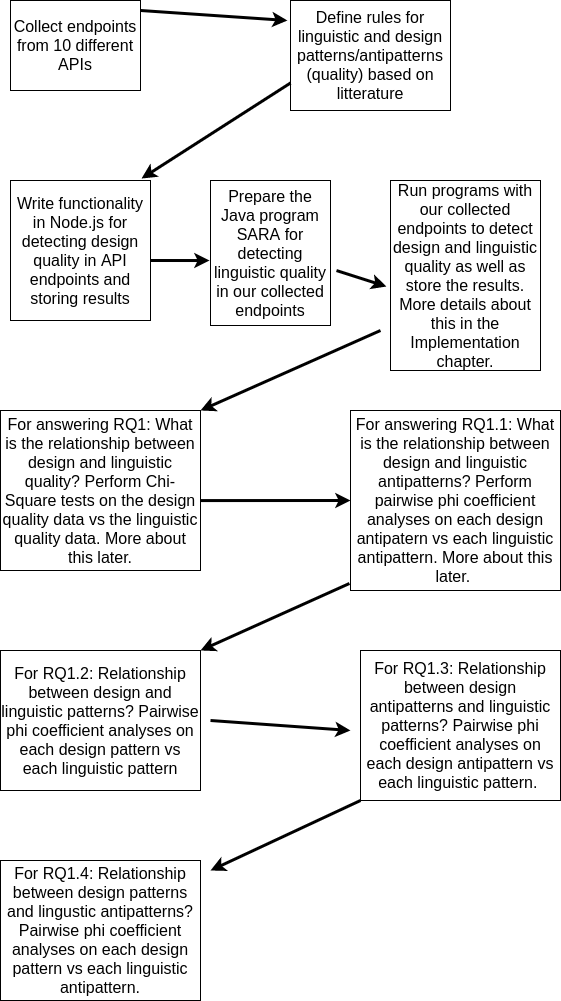
\includegraphics[scale=0.6]{Template_report_LaTeX_EN/img/method_figures/method_figure.png}
    \caption{Method figure}
    \label{fig:Method figure}
\end{figure}

We created a Node.js program for making HTTP requests to the selected API endpoints and check for REST design antipatterns. For detecting linguistic antipatterns the Java program created by Palma et al. for their study of linguistic REST antipatterns \cite{linguistic} for checking for those types of antipatterns in the endpoints will be used. TODO: reference figures

TODO: write about other programs, code used

\begin{figure}[htb!]
    \centering
    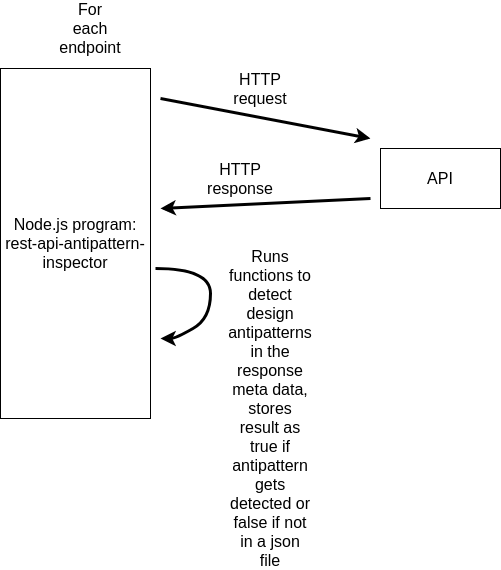
\includegraphics[scale=0.6]{Template_report_LaTeX_EN/img/method_figures/rest-api-antipattern-inspector.png}
    \caption{Detection of design antipatterns}
    \label{fig:Detection of design antipatterns}
\end{figure}

\begin{figure}[htb!]
    \centering
    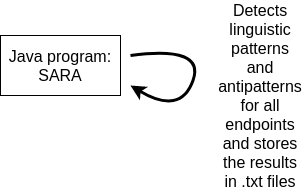
\includegraphics[scale=0.6]{Template_report_LaTeX_EN/img/method_figures/JAVA_SARA.png}
    \caption{Detection of linguistic quality}
    \label{fig:Detection of linguistic quality}
\end{figure}

\begin{figure}
    \centering
    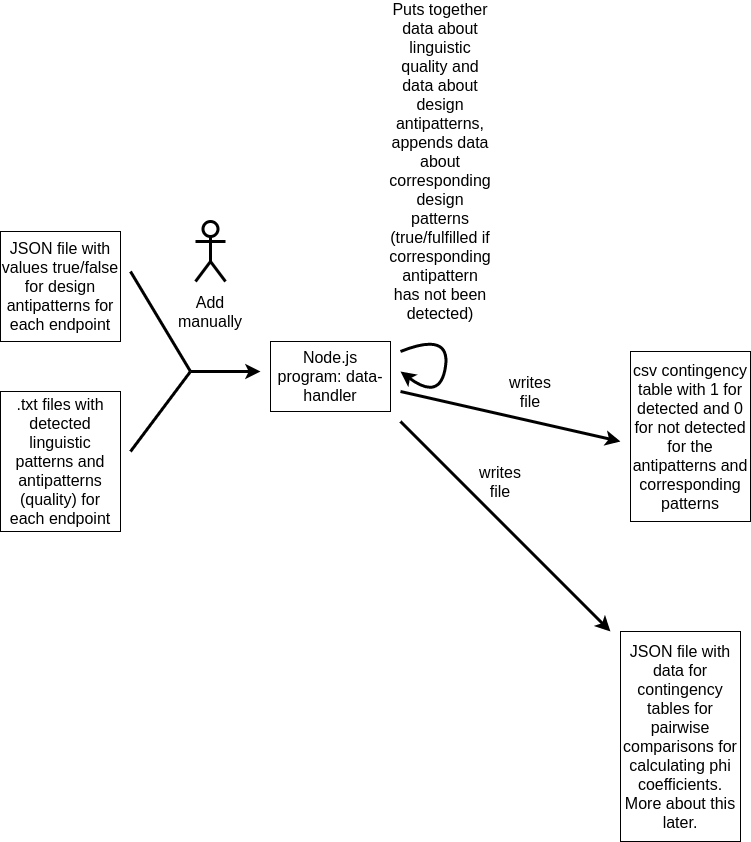
\includegraphics[scale=0.6]{Template_report_LaTeX_EN/img/method_figures/data_handler.png}
    \caption{Putting together the findings}
    \label{fig:Putting together the findings}
\end{figure}

\begin{figure}
    \centering
    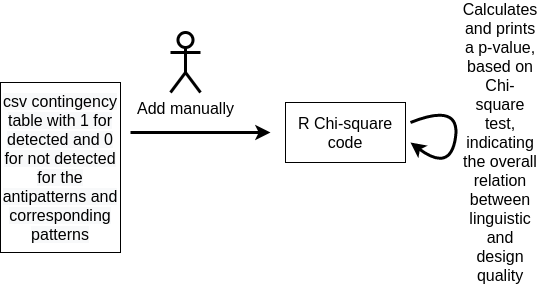
\includegraphics[scale=0.6]{Template_report_LaTeX_EN/img/method_figures/R_Chi_square.png}
    \caption{R chi square calculation}
    \label{fig:R chi square calculation}
\end{figure}

\begin{figure}
    \centering
    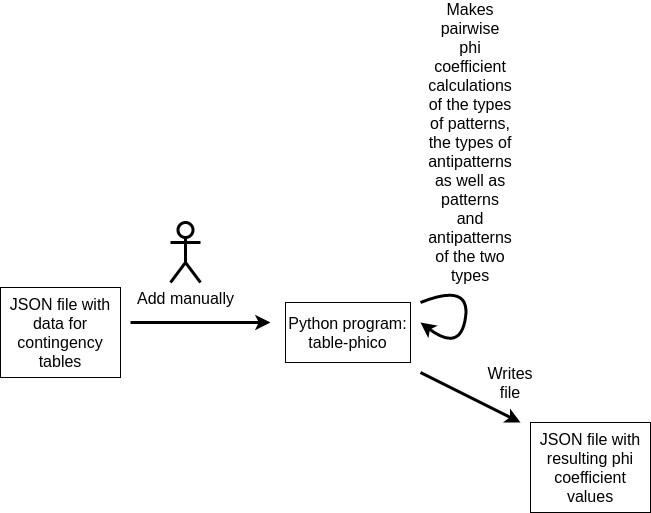
\includegraphics[scale=0.6]{Template_report_LaTeX_EN/img/method_figures/table_phico.png}
    \caption{Calculation of phi coefficients}
    \label{fig:Calculation of phi coefficients}
\end{figure}

\clearpage

\subsection{Reliability and Validity}
To increase reliability the study includes several appendixes, for example links to repositories/downloads of the source code used (with documentation for how to use it), as well as a document of all the API endpoints used. This will make it possible for others to recreate and inspect the research conducted. Unit tests are exists for the antipattern detection methods in the Node.js program for detecting REST design antipatterns. 
One reliability risk is that the API versions used might become outdated and replaced with new versions. The API versions used have therefore been listed to let future researchers that might want to replicate our findings know which API versions were used. Hopefully the API versions we used will still be supported. 
Another reliability risk is that the APIs could fix some errors detected which could produce different results if the detection programs used in this study are used again in the future. However, large changes within an API version should be unlikely. 
The biggest challenge will be to achieve a high validity. Time is a limited resource, there are limits to the amount of APIs that can be inspected and how many endpoints can be inspected in those. The  selection of APIs will be based on previous research by Palma et al. \cite{linguistic} and Google APIs will be excluded from them. From those APIs endpoints will be prioritized that have unique qualities and are prominent in the documentation. 
Another threat to validity is that our findings might become less relevant if the problems found are fixed in later versions. However, even if the results would become significantly different in future versions, the result of this study would still provide a snapshot of current conditions. 

\newpage

\section{Implementation}

\subsection{Detection of linguistic antipatterns}
Semantic analysis of RESTful APIs (SARA) is a program used for detecting linguistic antipatterns in URIs of RESTful APIs introduced by the research of Palma et al. \cite{linguistic}. SARA builds on a previous project DOLAR - Detection of Linguistic Antipatterns in REST - with the extended functionality to detect contextless resources, inconsistent documentation and less cohesive documentation.
Our research will use SARA for detecting the following linguistic antipatterns:
\begin{itemize}
\item Amorphous URIs
\item CRUDY URIs
\item Non-hierarchical Nodes
\item Inconsistent use of Singularised/Pluralised Nodes
\item Contextless Resource Names
\end{itemize}

The following antipatterns can be detected with SARA but will be excluded from our research:
\begin{itemize}
\item Unversioned URIs
\item Inconsistent documentation
\item Less cohesive documentation
\end{itemize}

SARA is built on JAVA and runs in the console. Each API is run separately and the result is stored in textfiles. Each text file consists of a list with URIs that are antipatterns and URI that passed the test.
The linguistic program has been further developed to get a more accurate result from finding contextless resources/URIs. Previously there was a limitation where nodes in an uri had words written together like “districtheat” where the following URI would become an antipattern: 

/v3/{agreementId}/consumption/districtheat/data

With our improvement the program can detect words written together and treat them as separate nodes. If a word is not found in the dictionary then this code block is executed to check if the word might consist of more than one word. The two new words must make use of all the characters of the old word.

\subsection{Detection of REST design antipatterns}

To be able to detect REST design antipatterns in APIs, we have developed a program for automatically making API calls, analyzing the metadata and storing the results. 
The program for detecting REST design antipatterns is written in TypeScript using the Node.js platform. These techniques were chosen partly because JavaScript is the most used language on Github \cite{octogithub} and because TypeScript, which extends JavaScript \cite{typescript}, is among the fastest growing languages on Github \cite{octogithub}. The aim is that this choice of techniques will help make our source code understandable for a wide audience. It is desirable for the sake of increased reliability for other developers and researchers to be able to understand our source code and thereby be able to validate it. Working with techniques that are currently commonly used will also result in access to many modern third party software libraries which will simplify and speed up the development process as well as reduce the risk of flaws since software libraries that are commonly used, have been battle-tested and have gotten good reviews can be selected. In addition, Node.js was selected for its suitability for handling HTTP calls \cite{nodejs} and TypeScript was selected to help with the detection of flaws \cite{typescript} in the development of the source code. 
The program has a Command Line Interface (CLI), the user selects which APIs to run detections for and the results with meta data gets stored in a JSON file. 

\subsection{Design Antipattern Detection functions}

The function below is designed to detect the Breaking Self-descriptiveness antipattern, this functions and many of our other functions uses helper functions we have created in other parts of the source code, it returns the boolean value true if the antipattern is detected and false otherwise:

\begin{center}
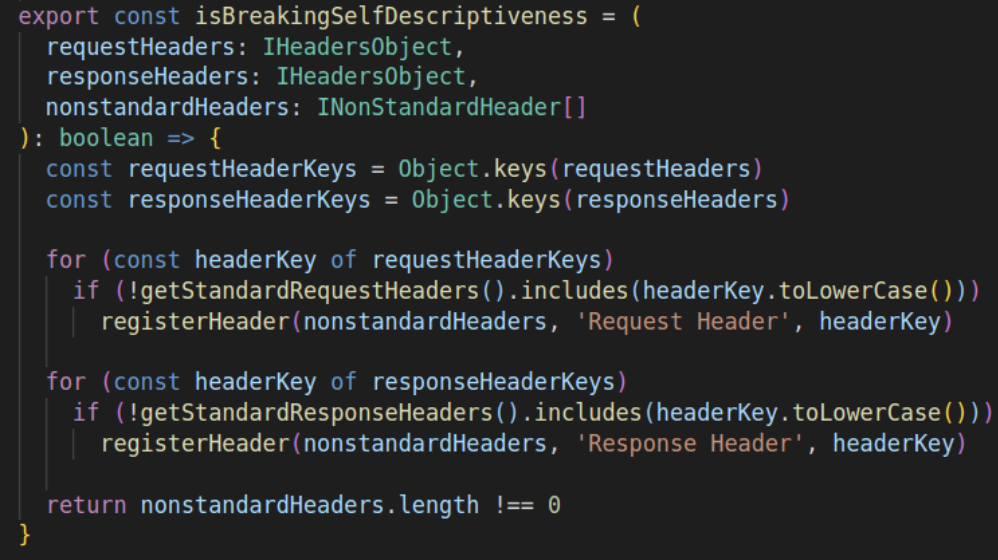
\includegraphics[keepaspectratio,scale=0.8]{Template_report_LaTeX_EN/img/breakingSelfDescriptiveness.png}
Figure 3.1: antipattern Breaking Self-descriptiveness gets detected if there are any non-standard headers in the request or response headers after an API call. 
\end{center}

\begin{center}
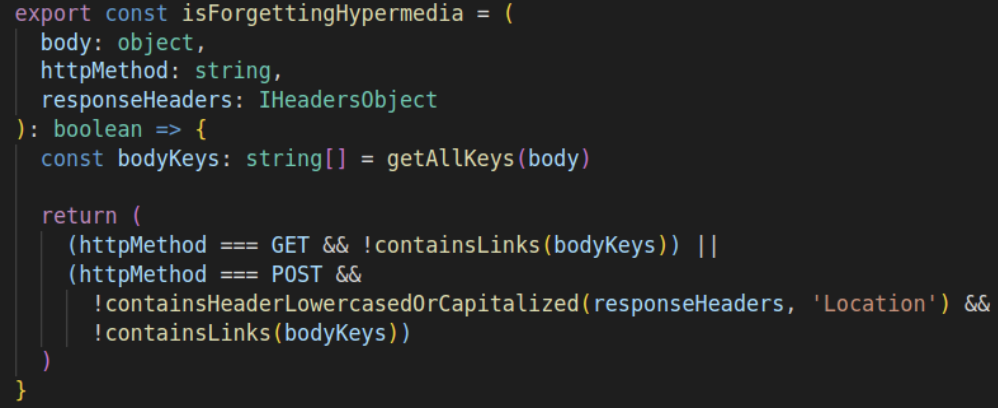
\includegraphics[keepaspectratio,scale=0.8]{Template_report_LaTeX_EN/img/forgettingHyperMedia.png}
Figure 3.2: antipattern Forgetting Hypermedia gets detected if the response body to a GET request does not contain any link keys (link/links/href) or if a POST request does not contain that or a Location header.
\end{center}

\begin{center}
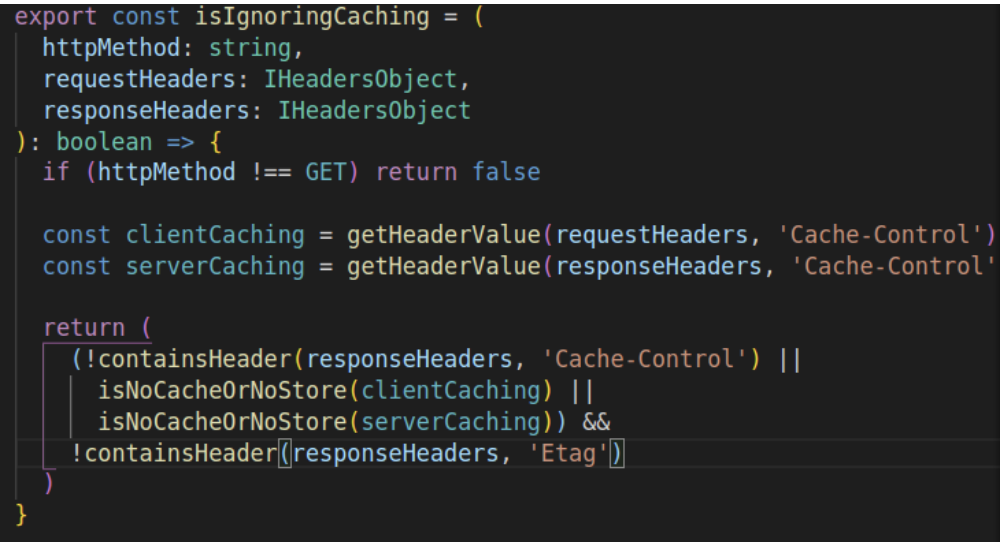
\includegraphics[keepaspectratio,scale=0.8]{Template_report_LaTeX_EN/img/ignoringCaching.png}
Figure 3.3: antipattern Ignoring Caching gets detected for responses to GET requests if the response headers do not contain an Etag or if the request or response headers does not contain a Cache-Control header or if that is set to "no-cache"/"no-store". 
\end{center}

\begin{center}
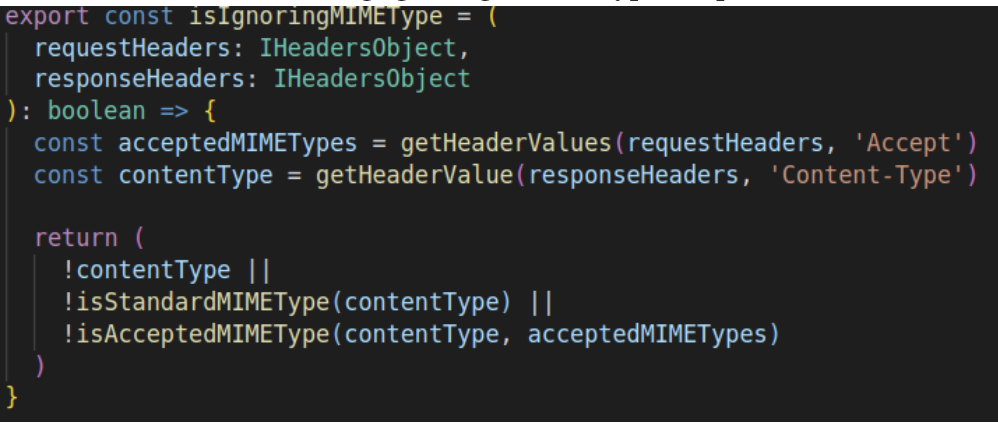
\includegraphics[keepaspectratio,scale=0.8]{Template_report_LaTeX_EN/img/ignoringMimeType.png}
Figure 3.4: antipattern Ignoring MIME Types gets detected if the response Content-Type header's value is not a standard mime type or if it is not among the accepted mime types requested. 
\end{center}

\begin{center}
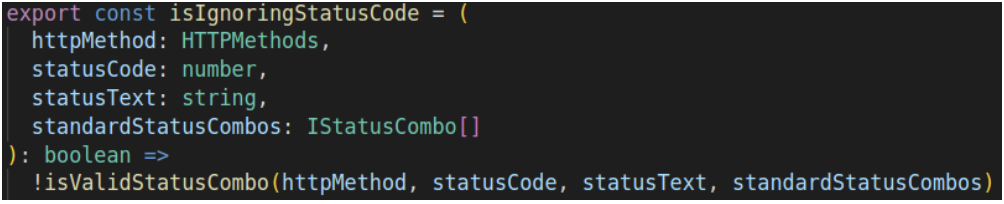
\includegraphics[keepaspectratio,scale=0.8]{Template_report_LaTeX_EN/img/ignoringStatusCode.png}
Figure 3.5: If the HTTP method used is GET, POST, PUT or DELETE: antipattern Ignoring Status Code gets detected if the combination of HTTP method, status code and status text in the response is not part of a list of valid combinations in an XML file used in the implementation by Palma et. al \cite{linguistic}.
\end{center}

\begin{center}
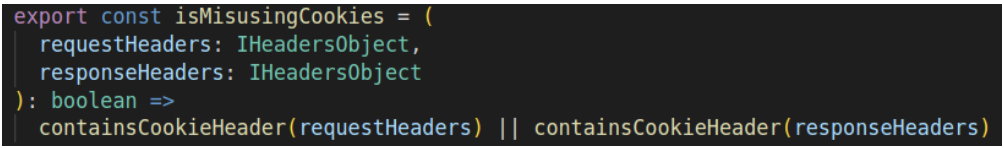
\includegraphics[keepaspectratio,scale=0.8]{Template_report_LaTeX_EN/img/misusingCookies.png}
Figure 3.6: antipattern Misusing Cookies gets detected if the request or response headers contain any type of cookie header. 
\end{center}

\subsection{Detection of patterns}

After detecting antipatterns and storing meta data about them, this function is used to determine and store information about patterns in our Node.js data-handler program. The patterns are set to true, meaning they are fulfilled, if the corresponding antipatterns are set to false, meaning no such antipattern was detected\footnote{https://github.com/rest-api-antipattern-inspector/data-handler}:

\begin{center}
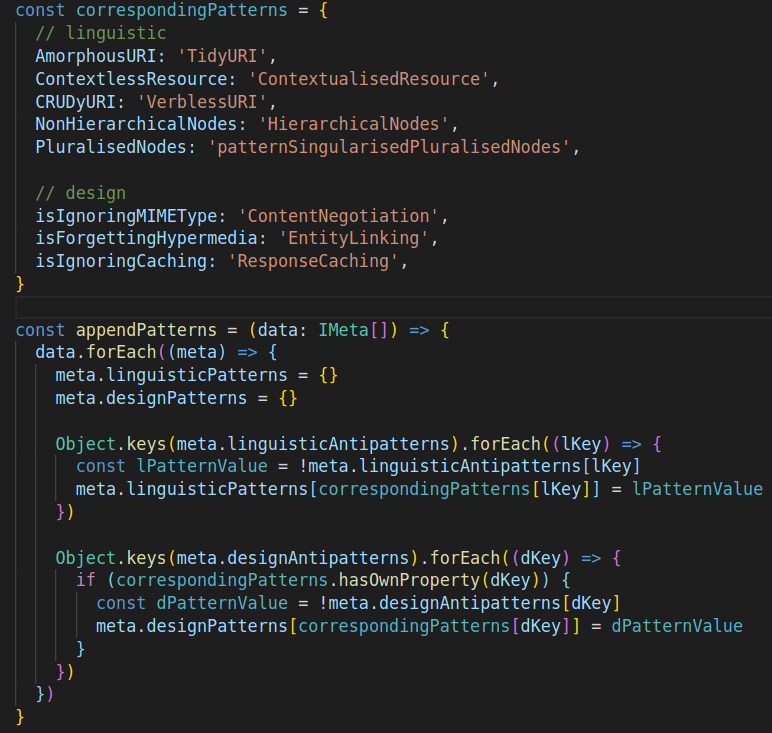
\includegraphics[keepaspectratio,scale=0.6]{Template_report_LaTeX_EN/img/patternsFunction.png}
\end{center}

\subsection{Calculating the correlations}

We have also written a program in TypeScript using Node.js for calculating the correlations between the linguistic and design antipatterns. 

\newpage

\section{Results}

\subsection{\textbf{RQ1:} What is the relationship between design quality and linguistic quality in RESTful APIs?}

\begin{table}[ht!]
\scriptsize
\begin{tabular}{|p{15mm}|p{9mm}|p{9mm}|p{9mm}|p{9mm}|p{9mm}|p{9mm}|p{9mm}|p{9mm}|p{9mm}|p{9mm}|}
\hline Antipatterns & Amor\-phous URI & CRUDy URI & Context\-less Resource & Pluralised Nodes& Non-hiera\-rchical Nodes & Tidy URI & Verbless URI & Context\-ualised Resource & Pluralised Nodes Pattern& Hierar\-chical Nodes  \\
\hline 
 Breaking Self-descriptiveness &
 36 &
 28 &
 53 &
 39 &
 0 &
 281 &
 289 &
 264 &
 278 &
 317
\\ \hline
 Forgetting Hypermedia &
 0 &
 0 &
 0 &
 0 &
 0 &
 0 &
 0 &
 0 &
 0 &
 0
\\ \hline
 Misusing Cookies &
 0 &
 24 &
 14 &
 21 &
 0 &
 100 &
 76 &
 86 &
 79 &
 100
\\ \hline
Ignoring MIME Types &
 0 &
 0 &
 12 &
 6 &
 0 &
 89 &
 89 &
 77 &
 83 &
 89
\\ \hline
Ignoring Status Code &
 0 &
 1 &
 4 &
 0 &
 0 &
 4 &
 3 &
 0 &
 4 &
 4
\\ \hline
Ignoring Caching &
 0 &
 0 &
 0 &
 0 &
 0 &
 0 &
 0 &
 0 &
 0 &
 0
\\ \hline
Entity linking &
 36 &
 28 &
 57 &
 39 &
 0 &
 290 &
 298 &
 269 &
 287 &
 326
\\ \hline
Content negotiation &
 36 &
 28 &
 45 &
 33 &
 0 &
 201 &
 209 &
 192 &
 204 &
 237
\\ \hline
Response caching &
 36 &
 28 &
 57 &
 39 &
 0 &
 290 &
 298 &
 269 &
 287 &
 326
\\ \hline
\end{tabular}

\caption{Chi-square test on the set of design and linguistic patterns and antipatterns.}
\label{Chi-square test}
\end{table}

Table \ref{Chi-square test} shows the result of chi-square test using a contingency table over design and linguistic patterns and antipatterns equaled to \textbf{p-value = 2.28e-07} which indicates an overall strong relationship between linguistic and design quality. The chi-square test was performed in R-studio\footnote{https://www.rdocumentation.org/packages/stats/versions/3.6.2/topics/chisq.test} which has a built in functionality for this test. 

\clearpage

\subsection{\textbf{RQ1.1:} What is the relationship between design antipatterns and linguistic antipatterns in RESTful APIs?}

A total of 326 endpoints in 10 APIs were tested. This chart in figure \ref{fig:barchart} shows the percentage of each antipattern:

\begin{figure}[!h]
\begin{center}
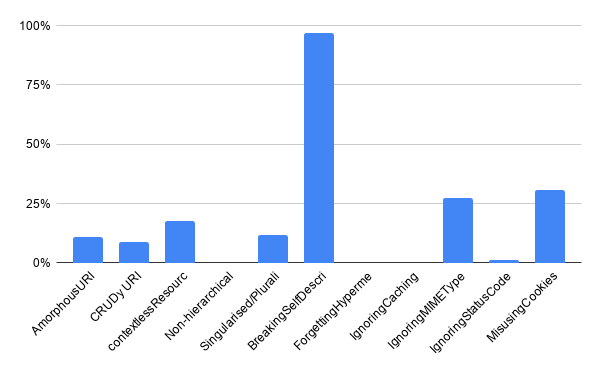
\includegraphics[keepaspectratio,scale=0.8]{Template_report_LaTeX_EN/img/bar_chart.png}
\caption{Shows how many endpoints had a specific antipattern in percentages.}
\label{fig:barchart}
\end{center}
\end{figure}

\begin{table}[hbt!]
    \centering
       \begin{tabular}{|p{90mm}|p{50mm}|}
\hline \textbf{Linguistic antipatterns vs Design antipatterns} & \textbf{Phi Coefficient} 
\\ \hline 
Amorphous URI vs Breaking Self-descriptiveness & 0.0593
\\ \hline
Amorphous URI vs Forgetting Hypermedia & NA
\\ \hline
Amorphous URI vs Ignoring Caching & NA
\\ \hline
Amorphous URI vs Ignoring MIME Types & -0.2159
\\ \hline
Amorphous URI vs Ignoring Status Code & -0.0392
\\ \hline
Amorphous URI vs Misusing Cookies & -0.2343
\\ \hline
CRUDy URI vs Breaking Self-descriptiveness & 0.0516
\\ \hline
CRUDy URI vs Forgetting Hypermedia & NA
\\ \hline
CRUDy URI vs Ignoring Caching & NA
\\ \hline
CRUDy URI vs Ignoring MIME Types & -0.1878
\\ \hline
CRUDy URI vs Ignoring Status Code & 0.0652
\\ \hline
CRUDy URI vs Misusing Cookies & 0.3658
\\ \hline
Contextless Resource vs Breaking Self-descriptiveness & -0.1195
\\ \hline
Contextless Resource vs Forgetting Hypermedia & NA
\\ \hline
Contextless Resource vs Ignoring Caching & NA
\\ \hline
Contextless Resource vs Ignoring MIME Types & -0.0645
\\ \hline
Contextless Resource vs Ignoring StatusCode & 0.2421
\\ \hline
Contextless Resource vs Misusing Cookies & -0.0610
\\ \hline
Non Hierarchical Nodes vs Breaking Self-descriptiveness & NA
\\ \hline
Non Hierarchical Nodes vs Forgetting Hypermedia & NA
\\ \hline
Non Hierarchical Nodes vs Ignoring Caching & NA
\\ \hline
Non Hierarchical Nodes vs Ignoring MIME Types & NA
\\ \hline
Non Hierarchical Nodes vs Ignoring StatusCode & NA
\\ \hline
Non Hierarchical Nodes vs Misusing Cookies & NA
\\ \hline
Pluralised Nodes vs Breaking Self-descriptiveness & 0.0621
\\ \hline
Pluralised Nodes vs Forgetting Hypermedia & NA
\\ \hline
Pluralised Nodes vs Ignoring Caching & NA
\\ \hline
Pluralised Nodes vs Ignoring MIME Types & -0.0985
\\ \hline
Pluralised Nodes vs Ignoring Status Code & -0.0410
\\ \hline
Pluralised Nodes vs Misusing Cookies & 0.1852
\\ \hline
    \end{tabular}
    \caption{Linguistic vs design antipatterns}
    \label{tab:Linguistic vs design antipatterns}
\end{table}

\clearpage

The result in table \ref{tab:Linguistic vs design antipatterns} indicates a moderate positive relation between the linguistic antipattern CRUDy URI and the design antipattern Misusing Cookies. It also indicates a weak positive relation between the linguistic antipattern Contextless Resource and the design antipattern Ignoring Status Code. 

Further indications of the result show that the linguistic antipattern Amorphous URI has a weak negative relation between both the design antipattern Misusing Cookies and the design antipattern Ignoring MIME Types. 

\subsection{\textbf{RQ1.2:} What is the relationship between design patterns and linguistic patterns in RESTful APIs?}

\begin{table}[hbt!]
    \centering
    \begin{tabular}{|p{90mm}|p{50mm}|}
\hline \textbf{Linguistic patterns vs Design patterns} & \textbf{Phi Coefficient} 
\\ \hline 
Tidy URI vs Entity Linking & NA
\\ \hline
Tidy URI vs Response Caching & NA
\\ \hline
Tidy URI vs Content Negotiation & -0.2159
\\ \hline
Verbless URI vs Entity Linking & NA
\\ \hline
Verbless URI vs Response Caching & NA
\\ \hline
Verbless URI vs Content Negotiation & -0.1878
\\ \hline
Contextualised Resource vs Entity Linking & NA
\\ \hline
Contextualised Resource vs Response Caching & NA
\\ \hline
Contextualised Resource vs Content Negotiation & -0.0645
\\ \hline
Hierarchical Nodes vs Entity Linking & NA
\\ \hline
Hierarchical Nodes vs Response Caching & NA
\\ \hline
Hierarchical Nodes vs Content Negotiation & NA
\\ \hline
Singularised Nodes vs EntityLinking & NA
\\ \hline
Singularised Nodes vs Response Caching & NA
\\ \hline
Singularised Nodes vs ContentNegotiation & -0.0985
\\ \hline
    \end{tabular}
    \caption{Linguistic vs design patterns}
    \label{tab:Linguistic vs design patterns}
\end{table}

\clearpage

Our result from table \ref{tab:Linguistic vs design patterns} indicate a weak negative relation between the design pattern Content Negotiation and the linguistic pattern Tidy URI. 

\subsection{\textbf{RQ1.3:} What is the relationship between design antipatterns and linguistic patterns in RESTful APIs?}

\begin{table}[htb!]
    \centering
   \begin{tabular}{|p{90mm}|p{50mm}|}
\hline \textbf{Linguistic patterns vs Design antipatterns} & \textbf{Phi Coefficient} 
\\ \hline 
Tidy URI vs Breaking Self-descriptiveness & -0.0593
\\ \hline 
Tidy URI vs Forgetting Hypermedia & NA
\\ \hline 
Tidy URI vs Ignoring Caching & NA
\\ \hline 
Tidy URI vs Ignoring MIME Types & 0.2159
\\ \hline 
Tidy URI vs Ignoring Status Code & 0.0392
\\ \hline 
Tidy URI vs Misusing Cookies & 0.2343
\\ \hline 
Verbless URI vs Breaking Self-descriptiveness & -0.0516
\\ \hline 
Verbless URI vs Forgetting Hypermedia & NA
\\ \hline 
Verbless URI vs Ignoring Caching & NA
\\ \hline 
Verbless URI vs Ignoring MIME Types & 0.1878
\\ \hline 
Verbless URI vs Ignoring Status Code & -0.0652
\\ \hline 
Verbless URI vs Misusing Cookies & -0.3658
\\ \hline 
Contextualised Resource vs Breaking Self-descriptiveness & 0.1195
\\ \hline 
Contextualised Resource vs Forgetting Hypermedia & NA
\\ \hline 
Contextualised Resource vs Ignoring Caching & NA
\\ \hline 
Contextualised Resource vs Ignoring MIME Types & 0.0645
\\ \hline 
Contextualised Resource vs Ignoring Status Code & -0.2421
\\ \hline 
Contextualised Resource vs Misusing Cookies & 0.0610
\\ \hline 
Hierarchical Nodes vs Breaking Self-descriptiveness & NA
\\ \hline 
Hierarchical Nodes vs Forgetting Hypermedia & NA
\\ \hline 
Hierarchical Nodes vs Ignoring Caching & NA
\\ \hline 
Hierarchical Nodes vs Ignoring MIME Types & NA
\\ \hline 
Hierarchical Nodes vs Ignoring Status Code & NA
\\ \hline 
Hierarchical Nodes vs Misusing Cookies & NA
\\ \hline 
Singularised Nodes vs Breaking Self-descriptiveness & -0.0621
\\ \hline 
Singularised Nodes vs Forgetting Hypermedia & NA
\\ \hline 
Singularised Nodes vs Ignoring Caching & NA
\\ \hline 
Singularised Nodes vs Ignoring MIME Types & 0.0985
\\ \hline 
Singularised Nodes vs Ignoring Status Code & 0.0410
\\ \hline 
Singularised Nodes vs Misusing Cookies & -0.1852
\\ \hline
    \end{tabular}
    \caption{Linguistic patterns vs design antipatterns}
    \label{tab:Linguistic patterns vs design antipatterns}
\end{table}

\clearpage

This result table of \ref{tab:Linguistic patterns vs design antipatterns} show a weak positive relations between the linguistic pattern Tidy URI and the design antipatterns Ignoring MIME Types and Misusing Cookies. 

Also a a moderate negative relation between the linguistic pattern Verbless URI and the design antipattern Misusing Cookies. Our result also indicates a weak negative relation between the linguistic pattern Contextualised Resource and the design antipattern Ignoring Status Code.

\subsection{\textbf{RQ1.4:} What is the relationship between design patterns and linguistic antipatterns in RESTful APIs?}

\begin{table}[hbt!]
    \centering
    \begin{tabular}{|p{90mm}|p{50mm}|}
\hline \textbf{Design patterns vs linguistic antipatterns} & \textbf{Phi Coefficient} 
\\ \hline 
Entity Linking vs Amorphous URI & NA
\\ \hline 
Entity Linking vs CRUDy URI & NA
\\ \hline 
Entity Linking vs Contextless Resource & NA
\\ \hline 
Entity Linking vs Non Hierarchical Nodes & NA
\\ \hline 
Entity Linking vs PluralisedNodes & NA
\\ \hline
Response Caching vs Amorphous URI & NA
\\ \hline 
Response Caching vs CRUDy URI & NA
\\ \hline 
Response Caching vs Contextless Resource & NA
\\ \hline 
Response Caching vs Non Hierarchical Nodes & NA
\\ \hline 
Response Caching vs PluralisedNodes & NA
\\ \hline
Content Negotiation vs Amorphous URI & 0.2159
\\ \hline 
Content Negotiation vs CRUDy URI & 0.1878
\\ \hline 
Content Negotiation vs Contextless Resource & 0.0645
\\ \hline 
Content Negotiation vs Non Hierarchical Nodes & NA
\\ \hline 
Content Negotiation vs Pluralised Nodes & 0.0985
\\ \hline 
    \end{tabular}
    \caption{Design patterns vs linguistic antipatterns}
    \label{tab:Design patterns vs linguistic antipatterns}
\end{table}

The result of table \ref{tab:Design patterns vs linguistic antipatterns} indicates a weak positive relation between the design pattern Content Negotiation and the linguistic antipattern Amorphous URI.

\clearpage

\newpage
	
\section{Analysis}

\subsection{RQ1: What is the relationship between design quality and linguistic quality inRESTful APIs?}

Based on chi square test there is a relationship between design and linguistic quality in REST APIs. The chi square test where a combination of antipatterns, patterns, and a mix of both.

\subsection{RQ1.1: What is the relationship between design antipatterns and linguistic an-tipatterns in RESTful APIs?}

According to the phi coefficient pairwise tests between the design and linguistic antipatterns there is a moderate positive relationship between CRUDy URI and misusing cookies. This is the strongest relation followed by a weak positive relationship for contextless resource vs ignoring status codes.

\subsection{RQ1.2:  What is the relationship between design patterns and linguistic patterns in RESTful APIs?}

We only define three patterns for REST design and two of these - Response caching and  entity linking - are present in every endpoint. In other words there where no corresponding antipattern detected. This most likely impacted this result. 

The results indicate a weak negative relation between the linguistic pattern Tidy URI and the design pattern Content Negotiation. Not much else can be said for this research question.

\subsection{ RQ1.3: What is the relationship between design antipatterns and linguistic patterns in RESTful APIs?}

We can see that there is an overall negative relationship between these two. If there are design antipatterns linguistic pattern seem to be less common also. As with research question 1.2 a lot of the pairwise tests could not bring any results.

\subsection{RQ1.4: What is the relationship between design patterns and linguistic antipatterns in RESTful APIs?}

Here we find a weak positive relationship in the pairwise phi coefficient tests between amorphous Uris and content negotiation.

\newpage
	
\section{Discussion}

\subsection{Antipattern analysis}

There a lot of endpoints breaking self descriptiveness (almost all of them except 4 in the Nasa API). From our result we can see a lot of APIs uses their own standard headers. A common custom header is for instance x-rate-limit that is common for a lot of the APIs and all their endpoints. It used for measuring how many request a client has made towards the API. 

The purpose of not inventing custom headers are so that developers using the API can understand the API better. They should not be forced to learn new rules and types of headers and their use case. Since so many endpoint had this antipattern one might question whether or not the rules for detecting these are to strict. For instance there might be a bigger fault to use a custom header if the purpose of this header is the same as a standard one. There are no standard header for determining the request limit towards an API so it might be the most natural solution to introduce a new custom header. Custom headers should always be prefixed by x-. 

There are no endpoints having the non-hierarchical nodes antipattern. Comparing our findings of linguistic antipatterns with Palma et al \cite{linguistic} we see that they measured as high as 56\% of the endpoints to contain the non-hierarchical nodes antipattern. We used the same program for detection SARA. There is a possibility that there might have been a change in the implementation since then which we are not aware of. Another possibility is that there is to few nodes (words between the slashes node1/node2) in our endpoints to measure any meaningful hierarchy.

\subsection{Patterns analysis}

There were no indications of relationships between design patterns and linguistic patterns, design patterns and linguistic antipatterns or linguistic patterns and design antipatterns. There where only a weak positive relationship between amorphous Uris and content negotiation. 

We defined 3 design patterns and 5 linguistic patterns. Since two out of three of the design patterns - Response caching and entity linking - had 100\% coverage of the endpoints tested the result wont yield any strong relations. Since content negotiation was the only design pattern which did not have 100\% coverage it was the only one that could bring any meaningful relations when running the phi coefficient tests. They also had a weak positive relation with amorphous URIs.

Since hierarchical nodes are determined by non-hierarchical nodes antipattern reversed there might be a different result from this if we investigate the reliability of the detection method. As mentioned in previous subsection the SARA algorithm for detecting this antipattern might no longer work as expected since previous research by Palma et al \cite{linguistic} showed a much higher detection for this antipattern.

For entity linking which looks for relational resources to an endpoint yielded no antipatterns (forgetting hypermedia). This pattern also had a 100\% coverage. There might be reason to see if the detection of the antipattern is to loose. This is one of the harder antipatterns to detect by scripting so there might be reason to verify these results manually. 

Ignoring caching was not detected as an antipattern and so the response caching pattern had a 100\% coverage. That all the APIs seem to conform to standard caching techniques might be less surprising since no public API want to be burdened by unnecessary requests.  
\newpage
		
\section{Conclusion}

By defining a set of rules for detecting patterns and antipatterns in REST APIs to find a relationship between linguistic and design quality we have produced results that covered 327 endpoints over 10 mayor APIs. 

The purpose of the research has been to increase the awareness of these quality issues for those who develops REST APIs, and mainly public REST API that other developers uses to integrate in their applications. 

We identified a moderate relationship between CRUDy URIs and misusing cookies. There where a weak positive relationship between amorphous Uris vs content negotiation, contextless resource vs ignoring status codes.

To make our result more reliable there is a need for verifying some of the detection methods used. Most notably non-hierarchical nodes and forgetting hypermedia. The reason for this is that forgetting hypermedia is hard to make a 100\% good script for detection of this antipattern. Looking for object keys in the body that contains "url","links" and their synonyms might be to loose since these fields could contain values that do not point to other resources within the API. 

Since our detection of non-hierarchical nodes differed so much from Palma et al\cite{linguistic} result there must be a raised concerned that this detection algorithm might need some more verification before used. Or at least some investigation why they got such high detection rate using the same program.

Another way for making the results more reliable would be to include more APIs and endpoints. 327 endpoints where used in this study over 10 different APIs. There is another research being conducted that look for relation between linguistic quality and design quality in googles APIs. That study used its own methods for design antipattern detection. A comparison of their results with this research to validate each others detection functions could be made. Also the combined findings from both of these studies might produced a more accurate result.

\newpage


%----------------------------------------------------------------------------------------
%	References. IEEE style is used.
%
%----------------------------------------------------------------------------------------
\newpage


\hypersetup{urlcolor=black}
\bibliographystyle{IEEEtran}
\bibliography{referenser}
\newpage
%----------------------------------------------------------------------------------------
%	Appendix
%-----------------------------------------------------------------------------------------
\pagenumbering{Alph}
\setcounter{page}{1} % Reset page numbering for Appendix
\appendix

\section{Appendix 1} 
In the appendix you can put details that does not fit into the main report. Examples are source code, long tables with raw data and questionnaires.

\begin{center}
  \begin{tabular}{| p{60mm} | p{10mm} | p{35mm} | p{35mm} |}
  \hline
   & & \textbf{Breaking Self-descriptiveness} &
  \\
  \hline
  & & yes & no
  \\
  \hline
  \textbf{Tidy URIs} & yes & 281 & 9
  \\
  \hline
   & no & 36 & 0
  \\
  \hline
  \multicolumn{4}{|c|}{Result: Phi Coefficient = -0.0594, }
  \\ \hline
  \end{tabular}
  \end{center}

\begin{center}
  \begin{tabular}{| p{60mm} | p{10mm} | p{35mm} | p{35mm} |}
  \hline
   & & \textbf{Forgetting Hypermedia} &
  \\
  \hline
  & & yes & no
  \\
  \hline
  \textbf{Tidy URIs} & yes & 0 & 290
  \\
  \hline
   & no & 0 & 36
  \\
  \hline
  \multicolumn{4}{|c|}{Result: NA}
  \\ \hline
  \end{tabular}
  \end{center}

\begin{center}
  \begin{tabular}{| p{60mm} | p{10mm} | p{35mm} | p{35mm} |}
  \hline
   & & \textbf{Ignoring Caching} &
  \\
  \hline
  & & yes & no
  \\
  \hline
  \textbf{Tidy URIs} & yes & 0 & 290
  \\
  \hline
   & no & 0 & 36
  \\
  \hline
  \multicolumn{4}{|c|}{Result: NA}
  \\ \hline
  \end{tabular}
  \end{center}

\begin{center}
  \begin{tabular}{| p{60mm} | p{10mm} | p{35mm} | p{35mm} |}
  \hline
   & & \textbf{Ignoring MIME Types} &
  \\
  \hline
  & & yes & no
  \\
  \hline
  \textbf{Tidy URIs} & yes & 89 & 201
  \\
  \hline
   & no & 0 & 36
  \\
  \hline
  \multicolumn{4}{|c|}{Result: Phi Coefficient = 0.2159, }
  \\ \hline
  \end{tabular}
  \end{center}

\begin{center}
  \begin{tabular}{| p{60mm} | p{10mm} | p{35mm} | p{35mm} |}
  \hline
   & & \textbf{Ignoring Status Code} &
  \\
  \hline
  & & yes & no
  \\
  \hline
  \textbf{Tidy URIs} & yes & 4 & 286
  \\
  \hline
   & no & 0 & 36
  \\
  \hline
  \multicolumn{4}{|c|}{Result: Phi Coefficient = 0.0393, }
  \\ \hline
  \end{tabular}
  \end{center}

\begin{center}
  \begin{tabular}{| p{60mm} | p{10mm} | p{35mm} | p{35mm} |}
  \hline
   & & \textbf{Misusing Cookies} &
  \\
  \hline
  & & yes & no
  \\
  \hline
  \textbf{Tidy URIs} & yes & 100 & 190
  \\
  \hline
   & no & 0 & 36
  \\
  \hline
  \multicolumn{4}{|c|}{Result: Phi Coefficient = 0.2344, }
  \\ \hline
  \end{tabular}
  \end{center}

\begin{center}
  \begin{tabular}{| p{60mm} | p{10mm} | p{35mm} | p{35mm} |}
  \hline
   & & \textbf{Breaking Self-descriptiveness} &
  \\
  \hline
  & & yes & no
  \\
  \hline
  \textbf{Verbless URIs} & yes & 289 & 9
  \\
  \hline
   & no & 28 & 0
  \\
  \hline
  \multicolumn{4}{|c|}{Result: Phi Coefficient = -0.0516, }
  \\ \hline
  \end{tabular}
  \end{center}

\begin{center}
  \begin{tabular}{| p{60mm} | p{10mm} | p{35mm} | p{35mm} |}
  \hline
   & & \textbf{Forgetting Hypermedia} &
  \\
  \hline
  & & yes & no
  \\
  \hline
  \textbf{Verbless URIs} & yes & 0 & 298
  \\
  \hline
   & no & 0 & 28
  \\
  \hline
  \multicolumn{4}{|c|}{Result: NA}
  \\ \hline
  \end{tabular}
  \end{center}

\begin{center}
  \begin{tabular}{| p{60mm} | p{10mm} | p{35mm} | p{35mm} |}
  \hline
   & & \textbf{Ignoring Caching} &
  \\
  \hline
  & & yes & no
  \\
  \hline
  \textbf{Verbless URIs} & yes & 0 & 298
  \\
  \hline
   & no & 0 & 28
  \\
  \hline
  \multicolumn{4}{|c|}{Result: NA}
  \\ \hline
  \end{tabular}
  \end{center}

\begin{center}
  \begin{tabular}{| p{60mm} | p{10mm} | p{35mm} | p{35mm} |}
  \hline
   & & \textbf{Ignoring MIME Types} &
  \\
  \hline
  & & yes & no
  \\
  \hline
  \textbf{Verbless URIs} & yes & 89 & 209
  \\
  \hline
   & no & 0 & 28
  \\
  \hline
  \multicolumn{4}{|c|}{Result: Phi Coefficient = 0.1878, }
  \\ \hline
  \end{tabular}
  \end{center}

\begin{center}
  \begin{tabular}{| p{60mm} | p{10mm} | p{35mm} | p{35mm} |}
  \hline
   & & \textbf{Ignoring Status Code} &
  \\
  \hline
  & & yes & no
  \\
  \hline
  \textbf{Verbless URIs} & yes & 3 & 295
  \\
  \hline
   & no & 1 & 27
  \\
  \hline
  \multicolumn{4}{|c|}{Result: Phi Coefficient = -0.0653, }
  \\ \hline
  \end{tabular}
  \end{center}

\begin{center}
  \begin{tabular}{| p{60mm} | p{10mm} | p{35mm} | p{35mm} |}
  \hline
   & & \textbf{Misusing Cookies} &
  \\
  \hline
  & & yes & no
  \\
  \hline
  \textbf{Verbless URIs} & yes & 76 & 222
  \\
  \hline
   & no & 24 & 4
  \\
  \hline
  \multicolumn{4}{|c|}{Result: Phi Coefficient = -0.3659, }
  \\ \hline
  \end{tabular}
  \end{center}

\begin{center}
  \begin{tabular}{| p{60mm} | p{10mm} | p{35mm} | p{35mm} |}
  \hline
   & & \textbf{Breaking Self-descriptiveness} &
  \\
  \hline
  & & yes & no
  \\
  \hline
  \textbf{Contextualised Resource Names} & yes & 264 & 5
  \\
  \hline
   & no & 53 & 4
  \\
  \hline
  \multicolumn{4}{|c|}{Result: Phi Coefficient = 0.1196, }
  \\ \hline
  \end{tabular}
  \end{center}

\begin{center}
  \begin{tabular}{| p{60mm} | p{10mm} | p{35mm} | p{35mm} |}
  \hline
   & & \textbf{Forgetting Hypermedia} &
  \\
  \hline
  & & yes & no
  \\
  \hline
  \textbf{Contextualised Resource Names} & yes & 0 & 269
  \\
  \hline
   & no & 0 & 57
  \\
  \hline
  \multicolumn{4}{|c|}{Result: NA}
  \\ \hline
  \end{tabular}
  \end{center}

\begin{center}
  \begin{tabular}{| p{60mm} | p{10mm} | p{35mm} | p{35mm} |}
  \hline
   & & \textbf{Ignoring Caching} &
  \\
  \hline
  & & yes & no
  \\
  \hline
  \textbf{Contextualised Resource Names} & yes & 0 & 269
  \\
  \hline
   & no & 0 & 57
  \\
  \hline
  \multicolumn{4}{|c|}{Result: NA}
  \\ \hline
  \end{tabular}
  \end{center}

\begin{center}
  \begin{tabular}{| p{60mm} | p{10mm} | p{35mm} | p{35mm} |}
  \hline
   & & \textbf{Ignoring MIME Types} &
  \\
  \hline
  & & yes & no
  \\
  \hline
  \textbf{Contextualised Resource Names} & yes & 77 & 192
  \\
  \hline
   & no & 12 & 45
  \\
  \hline
  \multicolumn{4}{|c|}{Result: Phi Coefficient = 0.0646, }
  \\ \hline
  \end{tabular}
  \end{center}

\begin{center}
  \begin{tabular}{| p{60mm} | p{10mm} | p{35mm} | p{35mm} |}
  \hline
   & & \textbf{Ignoring Status Code} &
  \\
  \hline
  & & yes & no
  \\
  \hline
  \textbf{Contextualised Resource Names} & yes & 0 & 269
  \\
  \hline
   & no & 4 & 53
  \\
  \hline
  \multicolumn{4}{|c|}{Result: Phi Coefficient = -0.2421, }
  \\ \hline
  \end{tabular}
  \end{center}

\begin{center}
  \begin{tabular}{| p{60mm} | p{10mm} | p{35mm} | p{35mm} |}
  \hline
   & & \textbf{Misusing Cookies} &
  \\
  \hline
  & & yes & no
  \\
  \hline
  \textbf{Contextualised Resource Names} & yes & 86 & 183
  \\
  \hline
   & no & 14 & 43
  \\
  \hline
  \multicolumn{4}{|c|}{Result: Phi Coefficient = 0.0610, }
  \\ \hline
  \end{tabular}
  \end{center}

\begin{center}
  \begin{tabular}{| p{60mm} | p{10mm} | p{35mm} | p{35mm} |}
  \hline
   & & \textbf{Breaking Self-descriptiveness} &
  \\
  \hline
  & & yes & no
  \\
  \hline
  \textbf{Hierarchical Nodes} & yes & 317 & 9
  \\
  \hline
   & no & 0 & 0
  \\
  \hline
  \multicolumn{4}{|c|}{Result: NA}
  \\ \hline
  \end{tabular}
  \end{center}

\begin{center}
  \begin{tabular}{| p{60mm} | p{10mm} | p{35mm} | p{35mm} |}
  \hline
   & & \textbf{Forgetting Hypermedia} &
  \\
  \hline
  & & yes & no
  \\
  \hline
  \textbf{Hierarchical Nodes} & yes & 0 & 326
  \\
  \hline
   & no & 0 & 0
  \\
  \hline
  \multicolumn{4}{|c|}{Result: NA}
  \\ \hline
  \end{tabular}
  \end{center}

\begin{center}
  \begin{tabular}{| p{60mm} | p{10mm} | p{35mm} | p{35mm} |}
  \hline
   & & \textbf{Ignoring Caching} &
  \\
  \hline
  & & yes & no
  \\
  \hline
  \textbf{Hierarchical Nodes} & yes & 0 & 326
  \\
  \hline
   & no & 0 & 0
  \\
  \hline
  \multicolumn{4}{|c|}{Result: NA}
  \\ \hline
  \end{tabular}
  \end{center}

\begin{center}
  \begin{tabular}{| p{60mm} | p{10mm} | p{35mm} | p{35mm} |}
  \hline
   & & \textbf{Ignoring MIME Types} &
  \\
  \hline
  & & yes & no
  \\
  \hline
  \textbf{Hierarchical Nodes} & yes & 89 & 237
  \\
  \hline
   & no & 0 & 0
  \\
  \hline
  \multicolumn{4}{|c|}{Result: NA}
  \\ \hline
  \end{tabular}
  \end{center}

\begin{center}
  \begin{tabular}{| p{60mm} | p{10mm} | p{35mm} | p{35mm} |}
  \hline
   & & \textbf{Ignoring Status Code} &
  \\
  \hline
  & & yes & no
  \\
  \hline
  \textbf{Hierarchical Nodes} & yes & 4 & 322
  \\
  \hline
   & no & 0 & 0
  \\
  \hline
  \multicolumn{4}{|c|}{Result: NA}
  \\ \hline
  \end{tabular}
  \end{center}

\begin{center}
  \begin{tabular}{| p{60mm} | p{10mm} | p{35mm} | p{35mm} |}
  \hline
   & & \textbf{Misusing Cookies} &
  \\
  \hline
  & & yes & no
  \\
  \hline
  \textbf{Hierarchical Nodes} & yes & 100 & 226
  \\
  \hline
   & no & 0 & 0
  \\
  \hline
  \multicolumn{4}{|c|}{Result: NA}
  \\ \hline
  \end{tabular}
  \end{center}

\begin{center}
  \begin{tabular}{| p{60mm} | p{10mm} | p{35mm} | p{35mm} |}
  \hline
   & & \textbf{Breaking Self-descriptiveness} &
  \\
  \hline
  & & yes & no
  \\
  \hline
  \textbf{Singularised Nodes Pattern} & yes & 278 & 9
  \\
  \hline
   & no & 39 & 0
  \\
  \hline
  \multicolumn{4}{|c|}{Result: Phi Coefficient = -0.0621, }
  \\ \hline
  \end{tabular}
  \end{center}

\begin{center}
  \begin{tabular}{| p{60mm} | p{10mm} | p{35mm} | p{35mm} |}
  \hline
   & & \textbf{Forgetting Hypermedia} &
  \\
  \hline
  & & yes & no
  \\
  \hline
  \textbf{Singularised Nodes Pattern} & yes & 0 & 287
  \\
  \hline
   & no & 0 & 39
  \\
  \hline
  \multicolumn{4}{|c|}{Result: NA}
  \\ \hline
  \end{tabular}
  \end{center}

\begin{center}
  \begin{tabular}{| p{60mm} | p{10mm} | p{35mm} | p{35mm} |}
  \hline
   & & \textbf{Ignoring Caching} &
  \\
  \hline
  & & yes & no
  \\
  \hline
  \textbf{Singularised Nodes Pattern} & yes & 0 & 287
  \\
  \hline
   & no & 0 & 39
  \\
  \hline
  \multicolumn{4}{|c|}{Result: NA}
  \\ \hline
  \end{tabular}
  \end{center}

\begin{center}
  \begin{tabular}{| p{60mm} | p{10mm} | p{35mm} | p{35mm} |}
  \hline
   & & \textbf{Ignoring MIME Types} &
  \\
  \hline
  & & yes & no
  \\
  \hline
  \textbf{Singularised Nodes Pattern} & yes & 83 & 204
  \\
  \hline
   & no & 6 & 33
  \\
  \hline
  \multicolumn{4}{|c|}{Result: Phi Coefficient = 0.0986, }
  \\ \hline
  \end{tabular}
  \end{center}

\begin{center}
  \begin{tabular}{| p{60mm} | p{10mm} | p{35mm} | p{35mm} |}
  \hline
   & & \textbf{Ignoring Status Code} &
  \\
  \hline
  & & yes & no
  \\
  \hline
  \textbf{Singularised Nodes Pattern} & yes & 4 & 283
  \\
  \hline
   & no & 0 & 39
  \\
  \hline
  \multicolumn{4}{|c|}{Result: Phi Coefficient = 0.0411, }
  \\ \hline
  \end{tabular}
  \end{center}

\begin{center}
  \begin{tabular}{| p{60mm} | p{10mm} | p{35mm} | p{35mm} |}
  \hline
   & & \textbf{Misusing Cookies} &
  \\
  \hline
  & & yes & no
  \\
  \hline
  \textbf{Singularised Nodes Pattern} & yes & 79 & 208
  \\
  \hline
   & no & 21 & 18
  \\
  \hline
  \multicolumn{4}{|c|}{Result: Phi Coefficient = -0.1852, }
  \\ \hline
  \end{tabular}
  \end{center}

\begin{center}
  \begin{tabular}{| p{60mm} | p{10mm} | p{35mm} | p{35mm} |}
  \hline
   & & \textbf{Entity Linking} &
  \\
  \hline
  & & yes & no
  \\
  \hline
  \textbf{Tidy URIs} & yes & 290 & 0
  \\
  \hline
   & no & 36 & 0
  \\
  \hline
  \multicolumn{4}{|c|}{Result: NA}
  \\ \hline
  \end{tabular}
  \end{center}

\begin{center}
  \begin{tabular}{| p{60mm} | p{10mm} | p{35mm} | p{35mm} |}
  \hline
   & & \textbf{Response Caching} &
  \\
  \hline
  & & yes & no
  \\
  \hline
  \textbf{Tidy URIs} & yes & 290 & 0
  \\
  \hline
   & no & 36 & 0
  \\
  \hline
  \multicolumn{4}{|c|}{Result: NA}
  \\ \hline
  \end{tabular}
  \end{center}

\begin{center}
  \begin{tabular}{| p{60mm} | p{10mm} | p{35mm} | p{35mm} |}
  \hline
   & & \textbf{Content Negotiation} &
  \\
  \hline
  & & yes & no
  \\
  \hline
  \textbf{Tidy URIs} & yes & 201 & 89
  \\
  \hline
   & no & 36 & 0
  \\
  \hline
  \multicolumn{4}{|c|}{Result: Phi Coefficient = -0.2159, }
  \\ \hline
  \end{tabular}
  \end{center}

\begin{center}
  \begin{tabular}{| p{60mm} | p{10mm} | p{35mm} | p{35mm} |}
  \hline
   & & \textbf{Entity Linking} &
  \\
  \hline
  & & yes & no
  \\
  \hline
  \textbf{Verbless URIs} & yes & 298 & 0
  \\
  \hline
   & no & 28 & 0
  \\
  \hline
  \multicolumn{4}{|c|}{Result: NA}
  \\ \hline
  \end{tabular}
  \end{center}

\begin{center}
  \begin{tabular}{| p{60mm} | p{10mm} | p{35mm} | p{35mm} |}
  \hline
   & & \textbf{Response Caching} &
  \\
  \hline
  & & yes & no
  \\
  \hline
  \textbf{Verbless URIs} & yes & 298 & 0
  \\
  \hline
   & no & 28 & 0
  \\
  \hline
  \multicolumn{4}{|c|}{Result: NA}
  \\ \hline
  \end{tabular}
  \end{center}

\begin{center}
  \begin{tabular}{| p{60mm} | p{10mm} | p{35mm} | p{35mm} |}
  \hline
   & & \textbf{Content Negotiation} &
  \\
  \hline
  & & yes & no
  \\
  \hline
  \textbf{Verbless URIs} & yes & 209 & 89
  \\
  \hline
   & no & 28 & 0
  \\
  \hline
  \multicolumn{4}{|c|}{Result: Phi Coefficient = -0.1878, }
  \\ \hline
  \end{tabular}
  \end{center}

\begin{center}
  \begin{tabular}{| p{60mm} | p{10mm} | p{35mm} | p{35mm} |}
  \hline
   & & \textbf{Entity Linking} &
  \\
  \hline
  & & yes & no
  \\
  \hline
  \textbf{Contextualised Resource Names} & yes & 269 & 0
  \\
  \hline
   & no & 57 & 0
  \\
  \hline
  \multicolumn{4}{|c|}{Result: NA}
  \\ \hline
  \end{tabular}
  \end{center}

\begin{center}
  \begin{tabular}{| p{60mm} | p{10mm} | p{35mm} | p{35mm} |}
  \hline
   & & \textbf{Response Caching} &
  \\
  \hline
  & & yes & no
  \\
  \hline
  \textbf{Contextualised Resource Names} & yes & 269 & 0
  \\
  \hline
   & no & 57 & 0
  \\
  \hline
  \multicolumn{4}{|c|}{Result: NA}
  \\ \hline
  \end{tabular}
  \end{center}

\begin{center}
  \begin{tabular}{| p{60mm} | p{10mm} | p{35mm} | p{35mm} |}
  \hline
   & & \textbf{Content Negotiation} &
  \\
  \hline
  & & yes & no
  \\
  \hline
  \textbf{Contextualised Resource Names} & yes & 192 & 77
  \\
  \hline
   & no & 45 & 12
  \\
  \hline
  \multicolumn{4}{|c|}{Result: Phi Coefficient = -0.0646, }
  \\ \hline
  \end{tabular}
  \end{center}

\begin{center}
  \begin{tabular}{| p{60mm} | p{10mm} | p{35mm} | p{35mm} |}
  \hline
   & & \textbf{Entity Linking} &
  \\
  \hline
  & & yes & no
  \\
  \hline
  \textbf{Hierarchical Nodes} & yes & 326 & 0
  \\
  \hline
   & no & 0 & 0
  \\
  \hline
  \multicolumn{4}{|c|}{Result: NA}
  \\ \hline
  \end{tabular}
  \end{center}

\begin{center}
  \begin{tabular}{| p{60mm} | p{10mm} | p{35mm} | p{35mm} |}
  \hline
   & & \textbf{Response Caching} &
  \\
  \hline
  & & yes & no
  \\
  \hline
  \textbf{Hierarchical Nodes} & yes & 326 & 0
  \\
  \hline
   & no & 0 & 0
  \\
  \hline
  \multicolumn{4}{|c|}{Result: NA}
  \\ \hline
  \end{tabular}
  \end{center}

\begin{center}
  \begin{tabular}{| p{60mm} | p{10mm} | p{35mm} | p{35mm} |}
  \hline
   & & \textbf{Content Negotiation} &
  \\
  \hline
  & & yes & no
  \\
  \hline
  \textbf{Hierarchical Nodes} & yes & 237 & 89
  \\
  \hline
   & no & 0 & 0
  \\
  \hline
  \multicolumn{4}{|c|}{Result: NA}
  \\ \hline
  \end{tabular}
  \end{center}

\begin{center}
  \begin{tabular}{| p{60mm} | p{10mm} | p{35mm} | p{35mm} |}
  \hline
   & & \textbf{Entity Linking} &
  \\
  \hline
  & & yes & no
  \\
  \hline
  \textbf{Singularised Nodes Pattern} & yes & 287 & 0
  \\
  \hline
   & no & 39 & 0
  \\
  \hline
  \multicolumn{4}{|c|}{Result: NA}
  \\ \hline
  \end{tabular}
  \end{center}

\begin{center}
  \begin{tabular}{| p{60mm} | p{10mm} | p{35mm} | p{35mm} |}
  \hline
   & & \textbf{Response Caching} &
  \\
  \hline
  & & yes & no
  \\
  \hline
  \textbf{Singularised Nodes Pattern} & yes & 287 & 0
  \\
  \hline
   & no & 39 & 0
  \\
  \hline
  \multicolumn{4}{|c|}{Result: NA}
  \\ \hline
  \end{tabular}
  \end{center}

\begin{center}
  \begin{tabular}{| p{60mm} | p{10mm} | p{35mm} | p{35mm} |}
  \hline
   & & \textbf{Content Negotiation} &
  \\
  \hline
  & & yes & no
  \\
  \hline
  \textbf{Singularised Nodes Pattern} & yes & 204 & 83
  \\
  \hline
   & no & 33 & 6
  \\
  \hline
  \multicolumn{4}{|c|}{Result: Phi Coefficient = -0.0986, }
  \\ \hline
  \end{tabular}
  \end{center}

\begin{center}
  \begin{tabular}{| p{60mm} | p{10mm} | p{35mm} | p{35mm} |}
  \hline
   & & \textbf{Amorphous URIs} &
  \\
  \hline
  & & yes & no
  \\
  \hline
  \textbf{Entity Linking} & yes & 36 & 290
  \\
  \hline
   & no & 0 & 0
  \\
  \hline
  \multicolumn{4}{|c|}{Result: NA}
  \\ \hline
  \end{tabular}
  \end{center}

\begin{center}
  \begin{tabular}{| p{60mm} | p{10mm} | p{35mm} | p{35mm} |}
  \hline
   & & \textbf{CRUDy URIs} &
  \\
  \hline
  & & yes & no
  \\
  \hline
  \textbf{Entity Linking} & yes & 28 & 298
  \\
  \hline
   & no & 0 & 0
  \\
  \hline
  \multicolumn{4}{|c|}{Result: NA}
  \\ \hline
  \end{tabular}
  \end{center}

\begin{center}
  \begin{tabular}{| p{60mm} | p{10mm} | p{35mm} | p{35mm} |}
  \hline
   & & \textbf{Contextless Resource Names} &
  \\
  \hline
  & & yes & no
  \\
  \hline
  \textbf{Entity Linking} & yes & 57 & 269
  \\
  \hline
   & no & 0 & 0
  \\
  \hline
  \multicolumn{4}{|c|}{Result: NA}
  \\ \hline
  \end{tabular}
  \end{center}

\begin{center}
  \begin{tabular}{| p{60mm} | p{10mm} | p{35mm} | p{35mm} |}
  \hline
   & & \textbf{NonHierarchical Nodes} &
  \\
  \hline
  & & yes & no
  \\
  \hline
  \textbf{Entity Linking} & yes & 0 & 326
  \\
  \hline
   & no & 0 & 0
  \\
  \hline
  \multicolumn{4}{|c|}{Result: NA}
  \\ \hline
  \end{tabular}
  \end{center}

\begin{center}
  \begin{tabular}{| p{60mm} | p{10mm} | p{35mm} | p{35mm} |}
  \hline
   & & \textbf{PluralisedNodes} &
  \\
  \hline
  & & yes & no
  \\
  \hline
  \textbf{Entity Linking} & yes & 39 & 287
  \\
  \hline
   & no & 0 & 0
  \\
  \hline
  \multicolumn{4}{|c|}{Result: NA}
  \\ \hline
  \end{tabular}
  \end{center}

\begin{center}
  \begin{tabular}{| p{60mm} | p{10mm} | p{35mm} | p{35mm} |}
  \hline
   & & \textbf{Amorphous URIs} &
  \\
  \hline
  & & yes & no
  \\
  \hline
  \textbf{Response Caching} & yes & 36 & 290
  \\
  \hline
   & no & 0 & 0
  \\
  \hline
  \multicolumn{4}{|c|}{Result: NA}
  \\ \hline
  \end{tabular}
  \end{center}

\begin{center}
  \begin{tabular}{| p{60mm} | p{10mm} | p{35mm} | p{35mm} |}
  \hline
   & & \textbf{CRUDy URIs} &
  \\
  \hline
  & & yes & no
  \\
  \hline
  \textbf{Response Caching} & yes & 28 & 298
  \\
  \hline
   & no & 0 & 0
  \\
  \hline
  \multicolumn{4}{|c|}{Result: NA}
  \\ \hline
  \end{tabular}
  \end{center}

\begin{center}
  \begin{tabular}{| p{60mm} | p{10mm} | p{35mm} | p{35mm} |}
  \hline
   & & \textbf{Contextless Resource Names} &
  \\
  \hline
  & & yes & no
  \\
  \hline
  \textbf{Response Caching} & yes & 57 & 269
  \\
  \hline
   & no & 0 & 0
  \\
  \hline
  \multicolumn{4}{|c|}{Result: NA}
  \\ \hline
  \end{tabular}
  \end{center}

\begin{center}
  \begin{tabular}{| p{60mm} | p{10mm} | p{35mm} | p{35mm} |}
  \hline
   & & \textbf{NonHierarchical Nodes} &
  \\
  \hline
  & & yes & no
  \\
  \hline
  \textbf{Response Caching} & yes & 0 & 326
  \\
  \hline
   & no & 0 & 0
  \\
  \hline
  \multicolumn{4}{|c|}{Result: NA}
  \\ \hline
  \end{tabular}
  \end{center}

\begin{center}
  \begin{tabular}{| p{60mm} | p{10mm} | p{35mm} | p{35mm} |}
  \hline
   & & \textbf{PluralisedNodes} &
  \\
  \hline
  & & yes & no
  \\
  \hline
  \textbf{Response Caching} & yes & 39 & 287
  \\
  \hline
   & no & 0 & 0
  \\
  \hline
  \multicolumn{4}{|c|}{Result: NA}
  \\ \hline
  \end{tabular}
  \end{center}

\begin{center}
  \begin{tabular}{| p{60mm} | p{10mm} | p{35mm} | p{35mm} |}
  \hline
   & & \textbf{Amorphous URIs} &
  \\
  \hline
  & & yes & no
  \\
  \hline
  \textbf{Content Negotiation} & yes & 36 & 201
  \\
  \hline
   & no & 0 & 89
  \\
  \hline
  \multicolumn{4}{|c|}{Result: Phi Coefficient = 0.2159, }
  \\ \hline
  \end{tabular}
  \end{center}

\begin{center}
  \begin{tabular}{| p{60mm} | p{10mm} | p{35mm} | p{35mm} |}
  \hline
   & & \textbf{CRUDy URIs} &
  \\
  \hline
  & & yes & no
  \\
  \hline
  \textbf{Content Negotiation} & yes & 28 & 209
  \\
  \hline
   & no & 0 & 89
  \\
  \hline
  \multicolumn{4}{|c|}{Result: Phi Coefficient = 0.1878, }
  \\ \hline
  \end{tabular}
  \end{center}

\begin{center}
  \begin{tabular}{| p{60mm} | p{10mm} | p{35mm} | p{35mm} |}
  \hline
   & & \textbf{Contextless Resource Names} &
  \\
  \hline
  & & yes & no
  \\
  \hline
  \textbf{Content Negotiation} & yes & 45 & 192
  \\
  \hline
   & no & 12 & 77
  \\
  \hline
  \multicolumn{4}{|c|}{Result: Phi Coefficient = 0.0646, }
  \\ \hline
  \end{tabular}
  \end{center}

\begin{center}
  \begin{tabular}{| p{60mm} | p{10mm} | p{35mm} | p{35mm} |}
  \hline
   & & \textbf{NonHierarchical Nodes} &
  \\
  \hline
  & & yes & no
  \\
  \hline
  \textbf{Content Negotiation} & yes & 0 & 237
  \\
  \hline
   & no & 0 & 89
  \\
  \hline
  \multicolumn{4}{|c|}{Result: NA}
  \\ \hline
  \end{tabular}
  \end{center}

\begin{center}
  \begin{tabular}{| p{60mm} | p{10mm} | p{35mm} | p{35mm} |}
  \hline
   & & \textbf{PluralisedNodes} &
  \\
  \hline
  & & yes & no
  \\
  \hline
  \textbf{Content Negotiation} & yes & 33 & 204
  \\
  \hline
   & no & 6 & 83
  \\
  \hline
  \multicolumn{4}{|c|}{Result: Phi Coefficient = 0.0986, }
  \\ \hline
  \end{tabular}
  \end{center}

\begin{center}
  \begin{tabular}{| p{60mm} | p{10mm} | p{35mm} | p{35mm} |}
  \hline
   & & \textbf{Breaking Self-descriptiveness} &
  \\
  \hline
  & & yes & no
  \\
  \hline
  \textbf{Amorphous URIs} & yes & 36 & 0
  \\
  \hline
   & no & 281 & 9
  \\
  \hline
  \multicolumn{4}{|c|}{Result: Phi Coefficient = 0.0594, }
  \\ \hline
  \end{tabular}
  \end{center}

\begin{center}
  \begin{tabular}{| p{60mm} | p{10mm} | p{35mm} | p{35mm} |}
  \hline
   & & \textbf{Forgetting Hypermedia} &
  \\
  \hline
  & & yes & no
  \\
  \hline
  \textbf{Amorphous URIs} & yes & 0 & 36
  \\
  \hline
   & no & 0 & 290
  \\
  \hline
  \multicolumn{4}{|c|}{Result: NA}
  \\ \hline
  \end{tabular}
  \end{center}

\begin{center}
  \begin{tabular}{| p{60mm} | p{10mm} | p{35mm} | p{35mm} |}
  \hline
   & & \textbf{Ignoring Caching} &
  \\
  \hline
  & & yes & no
  \\
  \hline
  \textbf{Amorphous URIs} & yes & 0 & 36
  \\
  \hline
   & no & 0 & 290
  \\
  \hline
  \multicolumn{4}{|c|}{Result: NA}
  \\ \hline
  \end{tabular}
  \end{center}

\begin{center}
  \begin{tabular}{| p{60mm} | p{10mm} | p{35mm} | p{35mm} |}
  \hline
   & & \textbf{Ignoring MIME Types} &
  \\
  \hline
  & & yes & no
  \\
  \hline
  \textbf{Amorphous URIs} & yes & 0 & 36
  \\
  \hline
   & no & 89 & 201
  \\
  \hline
  \multicolumn{4}{|c|}{Result: Phi Coefficient = -0.2159, }
  \\ \hline
  \end{tabular}
  \end{center}

\begin{center}
  \begin{tabular}{| p{60mm} | p{10mm} | p{35mm} | p{35mm} |}
  \hline
   & & \textbf{Ignoring Status Code} &
  \\
  \hline
  & & yes & no
  \\
  \hline
  \textbf{Amorphous URIs} & yes & 0 & 36
  \\
  \hline
   & no & 4 & 286
  \\
  \hline
  \multicolumn{4}{|c|}{Result: Phi Coefficient = -0.0393, }
  \\ \hline
  \end{tabular}
  \end{center}

\begin{center}
  \begin{tabular}{| p{60mm} | p{10mm} | p{35mm} | p{35mm} |}
  \hline
   & & \textbf{Misusing Cookies} &
  \\
  \hline
  & & yes & no
  \\
  \hline
  \textbf{Amorphous URIs} & yes & 0 & 36
  \\
  \hline
   & no & 100 & 190
  \\
  \hline
  \multicolumn{4}{|c|}{Result: Phi Coefficient = -0.2344, }
  \\ \hline
  \end{tabular}
  \end{center}

\begin{center}
  \begin{tabular}{| p{60mm} | p{10mm} | p{35mm} | p{35mm} |}
  \hline
   & & \textbf{Breaking Self-descriptiveness} &
  \\
  \hline
  & & yes & no
  \\
  \hline
  \textbf{CRUDy URIs} & yes & 28 & 0
  \\
  \hline
   & no & 289 & 9
  \\
  \hline
  \multicolumn{4}{|c|}{Result: Phi Coefficient = 0.0516, }
  \\ \hline
  \end{tabular}
  \end{center}

\begin{center}
  \begin{tabular}{| p{60mm} | p{10mm} | p{35mm} | p{35mm} |}
  \hline
   & & \textbf{Forgetting Hypermedia} &
  \\
  \hline
  & & yes & no
  \\
  \hline
  \textbf{CRUDy URIs} & yes & 0 & 28
  \\
  \hline
   & no & 0 & 298
  \\
  \hline
  \multicolumn{4}{|c|}{Result: NA}
  \\ \hline
  \end{tabular}
  \end{center}

\begin{center}
  \begin{tabular}{| p{60mm} | p{10mm} | p{35mm} | p{35mm} |}
  \hline
   & & \textbf{Ignoring Caching} &
  \\
  \hline
  & & yes & no
  \\
  \hline
  \textbf{CRUDy URIs} & yes & 0 & 28
  \\
  \hline
   & no & 0 & 298
  \\
  \hline
  \multicolumn{4}{|c|}{Result: NA}
  \\ \hline
  \end{tabular}
  \end{center}

\begin{center}
  \begin{tabular}{| p{60mm} | p{10mm} | p{35mm} | p{35mm} |}
  \hline
   & & \textbf{Ignoring MIME Types} &
  \\
  \hline
  & & yes & no
  \\
  \hline
  \textbf{CRUDy URIs} & yes & 0 & 28
  \\
  \hline
   & no & 89 & 209
  \\
  \hline
  \multicolumn{4}{|c|}{Result: Phi Coefficient = -0.1878, }
  \\ \hline
  \end{tabular}
  \end{center}

\begin{center}
  \begin{tabular}{| p{60mm} | p{10mm} | p{35mm} | p{35mm} |}
  \hline
   & & \textbf{Ignoring Status Code} &
  \\
  \hline
  & & yes & no
  \\
  \hline
  \textbf{CRUDy URIs} & yes & 1 & 27
  \\
  \hline
   & no & 3 & 295
  \\
  \hline
  \multicolumn{4}{|c|}{Result: Phi Coefficient = 0.0653, }
  \\ \hline
  \end{tabular}
  \end{center}

\begin{center}
  \begin{tabular}{| p{60mm} | p{10mm} | p{35mm} | p{35mm} |}
  \hline
   & & \textbf{Misusing Cookies} &
  \\
  \hline
  & & yes & no
  \\
  \hline
  \textbf{CRUDy URIs} & yes & 24 & 4
  \\
  \hline
   & no & 76 & 222
  \\
  \hline
  \multicolumn{4}{|c|}{Result: Phi Coefficient = 0.3659, }
  \\ \hline
  \end{tabular}
  \end{center}

\begin{center}
  \begin{tabular}{| p{60mm} | p{10mm} | p{35mm} | p{35mm} |}
  \hline
   & & \textbf{Breaking Self-descriptiveness} &
  \\
  \hline
  & & yes & no
  \\
  \hline
  \textbf{Contextless Resource Names} & yes & 53 & 4
  \\
  \hline
   & no & 264 & 5
  \\
  \hline
  \multicolumn{4}{|c|}{Result: Phi Coefficient = -0.1196, }
  \\ \hline
  \end{tabular}
  \end{center}

\begin{center}
  \begin{tabular}{| p{60mm} | p{10mm} | p{35mm} | p{35mm} |}
  \hline
   & & \textbf{Forgetting Hypermedia} &
  \\
  \hline
  & & yes & no
  \\
  \hline
  \textbf{Contextless Resource Names} & yes & 0 & 57
  \\
  \hline
   & no & 0 & 269
  \\
  \hline
  \multicolumn{4}{|c|}{Result: NA}
  \\ \hline
  \end{tabular}
  \end{center}

\begin{center}
  \begin{tabular}{| p{60mm} | p{10mm} | p{35mm} | p{35mm} |}
  \hline
   & & \textbf{Ignoring Caching} &
  \\
  \hline
  & & yes & no
  \\
  \hline
  \textbf{Contextless Resource Names} & yes & 0 & 57
  \\
  \hline
   & no & 0 & 269
  \\
  \hline
  \multicolumn{4}{|c|}{Result: NA}
  \\ \hline
  \end{tabular}
  \end{center}

\begin{center}
  \begin{tabular}{| p{60mm} | p{10mm} | p{35mm} | p{35mm} |}
  \hline
   & & \textbf{Ignoring MIME Types} &
  \\
  \hline
  & & yes & no
  \\
  \hline
  \textbf{Contextless Resource Names} & yes & 12 & 45
  \\
  \hline
   & no & 77 & 192
  \\
  \hline
  \multicolumn{4}{|c|}{Result: Phi Coefficient = -0.0646, }
  \\ \hline
  \end{tabular}
  \end{center}

\begin{center}
  \begin{tabular}{| p{60mm} | p{10mm} | p{35mm} | p{35mm} |}
  \hline
   & & \textbf{Ignoring Status Code} &
  \\
  \hline
  & & yes & no
  \\
  \hline
  \textbf{Contextless Resource Names} & yes & 4 & 53
  \\
  \hline
   & no & 0 & 269
  \\
  \hline
  \multicolumn{4}{|c|}{Result: Phi Coefficient = 0.2421, }
  \\ \hline
  \end{tabular}
  \end{center}

\begin{center}
  \begin{tabular}{| p{60mm} | p{10mm} | p{35mm} | p{35mm} |}
  \hline
   & & \textbf{Misusing Cookies} &
  \\
  \hline
  & & yes & no
  \\
  \hline
  \textbf{Contextless Resource Names} & yes & 14 & 43
  \\
  \hline
   & no & 86 & 183
  \\
  \hline
  \multicolumn{4}{|c|}{Result: Phi Coefficient = -0.0610, }
  \\ \hline
  \end{tabular}
  \end{center}

\begin{center}
  \begin{tabular}{| p{60mm} | p{10mm} | p{35mm} | p{35mm} |}
  \hline
   & & \textbf{Breaking Self-descriptiveness} &
  \\
  \hline
  & & yes & no
  \\
  \hline
  \textbf{NonHierarchical Nodes} & yes & 0 & 0
  \\
  \hline
   & no & 317 & 9
  \\
  \hline
  \multicolumn{4}{|c|}{Result: NA}
  \\ \hline
  \end{tabular}
  \end{center}

\begin{center}
  \begin{tabular}{| p{60mm} | p{10mm} | p{35mm} | p{35mm} |}
  \hline
   & & \textbf{Forgetting Hypermedia} &
  \\
  \hline
  & & yes & no
  \\
  \hline
  \textbf{NonHierarchical Nodes} & yes & 0 & 0
  \\
  \hline
   & no & 0 & 326
  \\
  \hline
  \multicolumn{4}{|c|}{Result: NA}
  \\ \hline
  \end{tabular}
  \end{center}

\begin{center}
  \begin{tabular}{| p{60mm} | p{10mm} | p{35mm} | p{35mm} |}
  \hline
   & & \textbf{Ignoring Caching} &
  \\
  \hline
  & & yes & no
  \\
  \hline
  \textbf{NonHierarchical Nodes} & yes & 0 & 0
  \\
  \hline
   & no & 0 & 326
  \\
  \hline
  \multicolumn{4}{|c|}{Result: NA}
  \\ \hline
  \end{tabular}
  \end{center}

\begin{center}
  \begin{tabular}{| p{60mm} | p{10mm} | p{35mm} | p{35mm} |}
  \hline
   & & \textbf{Ignoring MIME Types} &
  \\
  \hline
  & & yes & no
  \\
  \hline
  \textbf{NonHierarchical Nodes} & yes & 0 & 0
  \\
  \hline
   & no & 89 & 237
  \\
  \hline
  \multicolumn{4}{|c|}{Result: NA}
  \\ \hline
  \end{tabular}
  \end{center}

\begin{center}
  \begin{tabular}{| p{60mm} | p{10mm} | p{35mm} | p{35mm} |}
  \hline
   & & \textbf{Ignoring Status Code} &
  \\
  \hline
  & & yes & no
  \\
  \hline
  \textbf{NonHierarchical Nodes} & yes & 0 & 0
  \\
  \hline
   & no & 4 & 322
  \\
  \hline
  \multicolumn{4}{|c|}{Result: NA}
  \\ \hline
  \end{tabular}
  \end{center}

\begin{center}
  \begin{tabular}{| p{60mm} | p{10mm} | p{35mm} | p{35mm} |}
  \hline
   & & \textbf{Misusing Cookies} &
  \\
  \hline
  & & yes & no
  \\
  \hline
  \textbf{NonHierarchical Nodes} & yes & 0 & 0
  \\
  \hline
   & no & 100 & 226
  \\
  \hline
  \multicolumn{4}{|c|}{Result: NA}
  \\ \hline
  \end{tabular}
  \end{center}

\begin{center}
  \begin{tabular}{| p{60mm} | p{10mm} | p{35mm} | p{35mm} |}
  \hline
   & & \textbf{Breaking Self-descriptiveness} &
  \\
  \hline
  & & yes & no
  \\
  \hline
  \textbf{PluralisedNodes} & yes & 39 & 0
  \\
  \hline
   & no & 278 & 9
  \\
  \hline
  \multicolumn{4}{|c|}{Result: Phi Coefficient = 0.0621, }
  \\ \hline
  \end{tabular}
  \end{center}

\begin{center}
  \begin{tabular}{| p{60mm} | p{10mm} | p{35mm} | p{35mm} |}
  \hline
   & & \textbf{Forgetting Hypermedia} &
  \\
  \hline
  & & yes & no
  \\
  \hline
  \textbf{PluralisedNodes} & yes & 0 & 39
  \\
  \hline
   & no & 0 & 287
  \\
  \hline
  \multicolumn{4}{|c|}{Result: NA}
  \\ \hline
  \end{tabular}
  \end{center}

\begin{center}
  \begin{tabular}{| p{60mm} | p{10mm} | p{35mm} | p{35mm} |}
  \hline
   & & \textbf{Ignoring Caching} &
  \\
  \hline
  & & yes & no
  \\
  \hline
  \textbf{PluralisedNodes} & yes & 0 & 39
  \\
  \hline
   & no & 0 & 287
  \\
  \hline
  \multicolumn{4}{|c|}{Result: NA}
  \\ \hline
  \end{tabular}
  \end{center}

\begin{center}
  \begin{tabular}{| p{60mm} | p{10mm} | p{35mm} | p{35mm} |}
  \hline
   & & \textbf{Ignoring MIME Types} &
  \\
  \hline
  & & yes & no
  \\
  \hline
  \textbf{PluralisedNodes} & yes & 6 & 33
  \\
  \hline
   & no & 83 & 204
  \\
  \hline
  \multicolumn{4}{|c|}{Result: Phi Coefficient = -0.0986, }
  \\ \hline
  \end{tabular}
  \end{center}

\begin{center}
  \begin{tabular}{| p{60mm} | p{10mm} | p{35mm} | p{35mm} |}
  \hline
   & & \textbf{Ignoring Status Code} &
  \\
  \hline
  & & yes & no
  \\
  \hline
  \textbf{PluralisedNodes} & yes & 0 & 39
  \\
  \hline
   & no & 4 & 283
  \\
  \hline
  \multicolumn{4}{|c|}{Result: Phi Coefficient = -0.0411, }
  \\ \hline
  \end{tabular}
  \end{center}

\begin{center}
  \begin{tabular}{| p{60mm} | p{10mm} | p{35mm} | p{35mm} |}
  \hline
   & & \textbf{Misusing Cookies} &
  \\
  \hline
  & & yes & no
  \\
  \hline
  \textbf{PluralisedNodes} & yes & 21 & 18
  \\
  \hline
   & no & 79 & 208
  \\
  \hline
  \multicolumn{4}{|c|}{Result: Phi Coefficient = 0.1852, }
  \\ \hline
  \end{tabular}
  \end{center}


\end{document}

